\documentclass{llncs}
%%%%%%%%%%%%%%%%%%%%%%
%%%%   PACKAGES   %%%%
%%%%%%%%%%%%%%%%%%%%%%
\usepackage{makeidx}
\usepackage{amsmath}
\usepackage{amssymb}
\usepackage{stmaryrd}
\usepackage{graphicx}
\usepackage{subfigure}
\usepackage{latexsym}
\usepackage{url}
\usepackage{color}
\usepackage{isabelle}
\usepackage{isabellesym}
\usepackage{theorem}
\usepackage{algorithmic}
\usepackage[linesnumbered,ruled,vlined]{algorithm2e}
%\usepackage{program}
\usepackage{cases}

\newcommand\lyj[1]{\textcolor{red}{ #1} }

\newlength{\fminilength}
\newsavebox{\fminibox}
\newenvironment{fmini}[1][\linewidth]
  {\setlength{\fminilength}{#1\fboxsep-2\fboxrule}%
   \vspace{2ex}\noindent\begin{lrbox}{\fminibox}\begin{minipage}{\fminilength}%
   \mbox{ }\hfill\vspace{-2.5ex}}%
  {\end{minipage}\end{lrbox}\vspace{1ex}\hspace{0ex}%
   \framebox{\usebox{\fminibox}}}

\newenvironment{specification}
{\noindent\scriptsize
\tt\begin{fmini}\begin{tabbing}X\=X12345\=XXXX\=XXXX\=XXXX\=XXXX\=XXXX
\=\+\kill} {\end{tabbing}\normalfont\end{fmini}}
\def \twoSpaces {\ \ }
\def \oneSpace {\ }
\def \eqc {\doteq }
\def \andc {\barwedge }
\def \negc {!}
\def \orc {\veebar }
\def \alt {$/\backslash$ }
\def \cat {\symbol{94}}

\def \dbRight {$\backslash\backslash$}
\def \iInv {iInv}
\def \iR {iR}


% Macros for Scientific Word 2.5 documents saved with the LaTeX filter.
%Copyright (C) 1994-95 TCI Software Research, Inc.
\typeout{TCILATEX Macros for Scientific Word 2.5 <22 Dec 95>.}
\typeout{NOTICE:  This macro file is NOT proprietary and may be 
freely copied and distributed.}
%
\makeatletter
%
%%%%%%%%%%%%%%%%%%%%%%
% macros for time
\newcount\@hour\newcount\@minute\chardef\@x10\chardef\@xv60
\def\tcitime{
\def\@time{%
  \@minute\time\@hour\@minute\divide\@hour\@xv
  \ifnum\@hour<\@x 0\fi\the\@hour:%
  \multiply\@hour\@xv\advance\@minute-\@hour
  \ifnum\@minute<\@x 0\fi\the\@minute
  }}%

%%%%%%%%%%%%%%%%%%%%%%
% macro for hyperref
\@ifundefined{hyperref}{\def\hyperref#1#2#3#4{#2\ref{#4}#3}}{}

% macro for external program call
\@ifundefined{qExtProgCall}{\def\qExtProgCall#1#2#3#4#5#6{\relax}}{}
%%%%%%%%%%%%%%%%%%%%%%
%
% macros for graphics
%
\def\FILENAME#1{#1}%
%
\def\QCTOpt[#1]#2{%
  \def\QCTOptB{#1}
  \def\QCTOptA{#2}
}
\def\QCTNOpt#1{%
  \def\QCTOptA{#1}
  \let\QCTOptB\empty
}
\def\Qct{%
  \@ifnextchar[{%
    \QCTOpt}{\QCTNOpt}
}
\def\QCBOpt[#1]#2{%
  \def\QCBOptB{#1}
  \def\QCBOptA{#2}
}
\def\QCBNOpt#1{%
  \def\QCBOptA{#1}
  \let\QCBOptB\empty
}
\def\Qcb{%
  \@ifnextchar[{%
    \QCBOpt}{\QCBNOpt}
}
\def\PrepCapArgs{%
  \ifx\QCBOptA\empty
    \ifx\QCTOptA\empty
      {}%
    \else
      \ifx\QCTOptB\empty
        {\QCTOptA}%
      \else
        [\QCTOptB]{\QCTOptA}%
      \fi
    \fi
  \else
    \ifx\QCBOptA\empty
      {}%
    \else
      \ifx\QCBOptB\empty
        {\QCBOptA}%
      \else
        [\QCBOptB]{\QCBOptA}%
      \fi
    \fi
  \fi
}
\newcount\GRAPHICSTYPE
%\GRAPHICSTYPE 0 is for TurboTeX
%\GRAPHICSTYPE 1 is for DVIWindo (PostScript)
%%%(removed)%\GRAPHICSTYPE 2 is for psfig (PostScript)
\GRAPHICSTYPE=\z@
\def\GRAPHICSPS#1{%
 \ifcase\GRAPHICSTYPE%\GRAPHICSTYPE=0
   \special{ps: #1}%
 \or%\GRAPHICSTYPE=1
   \special{language "PS", include "#1"}%
%%%\or%\GRAPHICSTYPE=2
%%%  #1%
 \fi
}%
%
\def\GRAPHICSHP#1{\special{include #1}}%
%
% \graffile{ body }                                  %#1
%          { contentswidth (scalar)  }               %#2
%          { contentsheight (scalar) }               %#3
%          { vertical shift when in-line (scalar) }  %#4
\def\graffile#1#2#3#4{%
%%% \ifnum\GRAPHICSTYPE=\tw@
%%%  %Following if using psfig
%%%  \@ifundefined{psfig}{\input psfig.tex}{}%
%%%  \psfig{file=#1, height=#3, width=#2}%
%%% \else
  %Following for all others
  % JCS - added BOXTHEFRAME, see below
    \leavevmode
    \raise -#4 \BOXTHEFRAME{%
        \hbox to #2{\raise #3\hbox to #2{\null #1\hfil}}}%
}%
%
% A box for drafts
\def\draftbox#1#2#3#4{%
 \leavevmode\raise -#4 \hbox{%
  \frame{\rlap{\protect\tiny #1}\hbox to #2%
   {\vrule height#3 width\z@ depth\z@\hfil}%
  }%
 }%
}%
%
\newcount\draft
\draft=\z@
\let\nographics=\draft
\newif\ifwasdraft
\wasdraftfalse

%  \GRAPHIC{ body }                                  %#1
%          { draft name }                            %#2
%          { contentswidth (scalar)  }               %#3
%          { contentsheight (scalar) }               %#4
%          { vertical shift when in-line (scalar) }  %#5
\def\GRAPHIC#1#2#3#4#5{%
 \ifnum\draft=\@ne\draftbox{#2}{#3}{#4}{#5}%
  \else\graffile{#1}{#3}{#4}{#5}%
  \fi
 }%
%
\def\addtoLaTeXparams#1{%
    \edef\LaTeXparams{\LaTeXparams #1}}%
%
% JCS -  added a switch BoxFrame that can 
% be set by including X in the frame params.
% If set a box is drawn around the frame.

\newif\ifBoxFrame \BoxFramefalse
\newif\ifOverFrame \OverFramefalse
\newif\ifUnderFrame \UnderFramefalse

\def\BOXTHEFRAME#1{%
   \hbox{%
      \ifBoxFrame
         \frame{#1}%
      \else
         {#1}%
      \fi
   }%
}


\def\doFRAMEparams#1{\BoxFramefalse\OverFramefalse\UnderFramefalse\readFRAMEparams#1\end}%
\def\readFRAMEparams#1{%
 \ifx#1\end%
  \let\next=\relax
  \else
  \ifx#1i\dispkind=\z@\fi
  \ifx#1d\dispkind=\@ne\fi
  \ifx#1f\dispkind=\tw@\fi
  \ifx#1t\addtoLaTeXparams{t}\fi
  \ifx#1b\addtoLaTeXparams{b}\fi
  \ifx#1p\addtoLaTeXparams{p}\fi
  \ifx#1h\addtoLaTeXparams{h}\fi
  \ifx#1X\BoxFrametrue\fi
  \ifx#1O\OverFrametrue\fi
  \ifx#1U\UnderFrametrue\fi
  \ifx#1w
    \ifnum\draft=1\wasdrafttrue\else\wasdraftfalse\fi
    \draft=\@ne
  \fi
  \let\next=\readFRAMEparams
  \fi
 \next
 }%
%
%Macro for In-line graphics object
%   \IFRAME{ contentswidth (scalar)  }               %#1
%          { contentsheight (scalar) }               %#2
%          { vertical shift when in-line (scalar) }  %#3
%          { draft name }                            %#4
%          { body }                                  %#5
%          { caption}                                %#6


\def\IFRAME#1#2#3#4#5#6{%
      \bgroup
      \let\QCTOptA\empty
      \let\QCTOptB\empty
      \let\QCBOptA\empty
      \let\QCBOptB\empty
      #6%
      \parindent=0pt%
      \leftskip=0pt
      \rightskip=0pt
      \setbox0 = \hbox{\QCBOptA}%
      \@tempdima = #1\relax
      \ifOverFrame
          % Do this later
          \typeout{This is not implemented yet}%
          \show\HELP
      \else
         \ifdim\wd0>\@tempdima
            \advance\@tempdima by \@tempdima
            \ifdim\wd0 >\@tempdima
               \textwidth=\@tempdima
               \setbox1 =\vbox{%
                  \noindent\hbox to \@tempdima{\hfill\GRAPHIC{#5}{#4}{#1}{#2}{#3}\hfill}\\%
                  \noindent\hbox to \@tempdima{\parbox[b]{\@tempdima}{\QCBOptA}}%
               }%
               \wd1=\@tempdima
            \else
               \textwidth=\wd0
               \setbox1 =\vbox{%
                 \noindent\hbox to \wd0{\hfill\GRAPHIC{#5}{#4}{#1}{#2}{#3}\hfill}\\%
                 \noindent\hbox{\QCBOptA}%
               }%
               \wd1=\wd0
            \fi
         \else
            %\show\BBB
            \ifdim\wd0>0pt
              \hsize=\@tempdima
              \setbox1 =\vbox{%
                \unskip\GRAPHIC{#5}{#4}{#1}{#2}{0pt}%
                \break
                \unskip\hbox to \@tempdima{\hfill \QCBOptA\hfill}%
              }%
              \wd1=\@tempdima
           \else
              \hsize=\@tempdima
              \setbox1 =\vbox{%
                \unskip\GRAPHIC{#5}{#4}{#1}{#2}{0pt}%
              }%
              \wd1=\@tempdima
           \fi
         \fi
         \@tempdimb=\ht1
         \advance\@tempdimb by \dp1
         \advance\@tempdimb by -#2%
         \advance\@tempdimb by #3%
         \leavevmode
         \raise -\@tempdimb \hbox{\box1}%
      \fi
      \egroup%
}%
%
%Macro for Display graphics object
%   \DFRAME{ contentswidth (scalar)  }               %#1
%          { contentsheight (scalar) }               %#2
%          { draft label }                           %#3
%          { name }                                  %#4
%          { caption}                                %#5
\def\DFRAME#1#2#3#4#5{%
 \begin{center}
     \let\QCTOptA\empty
     \let\QCTOptB\empty
     \let\QCBOptA\empty
     \let\QCBOptB\empty
     \ifOverFrame 
        #5\QCTOptA\par
     \fi
     \GRAPHIC{#4}{#3}{#1}{#2}{\z@}
     \ifUnderFrame 
        \nobreak\par #5\QCBOptA
     \fi
 \end{center}%
 }%
%
%Macro for Floating graphic object
%   \FFRAME{ framedata f|i tbph x F|T }              %#1
%          { contentswidth (scalar)  }               %#2
%          { contentsheight (scalar) }               %#3
%          { caption }                               %#4
%          { label }                                 %#5
%          { draft name }                            %#6
%          { body }                                  %#7
\def\FFRAME#1#2#3#4#5#6#7{%
 \begin{figure}[#1]%
  \let\QCTOptA\empty
  \let\QCTOptB\empty
  \let\QCBOptA\empty
  \let\QCBOptB\empty
  \ifOverFrame
    #4
    \ifx\QCTOptA\empty
    \else
      \ifx\QCTOptB\empty
        \caption{\QCTOptA}%
      \else
        \caption[\QCTOptB]{\QCTOptA}%
      \fi
    \fi
    \ifUnderFrame\else
      \label{#5}%
    \fi
  \else
    \UnderFrametrue%
  \fi
  \begin{center}\GRAPHIC{#7}{#6}{#2}{#3}{\z@}\end{center}%
  \ifUnderFrame
    #4
    \ifx\QCBOptA\empty
      \caption{}%
    \else
      \ifx\QCBOptB\empty
        \caption{\QCBOptA}%
      \else
        \caption[\QCBOptB]{\QCBOptA}%
      \fi
    \fi
    \label{#5}%
  \fi
  \end{figure}%
 }%
%
%
%    \FRAME{ framedata f|i tbph x F|T }              %#1
%          { contentswidth (scalar)  }               %#2
%          { contentsheight (scalar) }               %#3
%          { vertical shift when in-line (scalar) }  %#4
%          { caption }                               %#5
%          { label }                                 %#6
%          { name }                                  %#7
%          { body }                                  %#8
%
%    framedata is a string which can contain the following
%    characters: idftbphxFT
%    Their meaning is as follows:
%             i, d or f : in-line, display, or floating
%             t,b,p,h   : LaTeX floating placement options
%             x         : fit contents box to contents
%             F or T    : Figure or Table. 
%                         Later this can expand
%                         to a more general float class.
%
%
\newcount\dispkind%

\def\makeactives{
  \catcode`\"=\active
  \catcode`\;=\active
  \catcode`\:=\active
  \catcode`\'=\active
  \catcode`\~=\active
}
\bgroup
   \makeactives
   \gdef\activesoff{%
      \def"{\string"}
      \def;{\string;}
      \def:{\string:}
      \def'{\string'}
      \def~{\string~}
      %\bbl@deactivate{"}%
      %\bbl@deactivate{;}%
      %\bbl@deactivate{:}%
      %\bbl@deactivate{'}%
    }
\egroup

\def\FRAME#1#2#3#4#5#6#7#8{%
 \bgroup
 \@ifundefined{bbl@deactivate}{}{\activesoff}
 \ifnum\draft=\@ne
   \wasdrafttrue
 \else
   \wasdraftfalse%
 \fi
 \def\LaTeXparams{}%
 \dispkind=\z@
 \def\LaTeXparams{}%
 \doFRAMEparams{#1}%
 \ifnum\dispkind=\z@\IFRAME{#2}{#3}{#4}{#7}{#8}{#5}\else
  \ifnum\dispkind=\@ne\DFRAME{#2}{#3}{#7}{#8}{#5}\else
   \ifnum\dispkind=\tw@
    \edef\@tempa{\noexpand\FFRAME{\LaTeXparams}}%
    \@tempa{#2}{#3}{#5}{#6}{#7}{#8}%
    \fi
   \fi
  \fi
  \ifwasdraft\draft=1\else\draft=0\fi{}%
  \egroup
 }%
%
% This macro added to let SW gobble a parameter that
% should not be passed on and expanded. 

\def\TEXUX#1{"texux"}

%
% Macros for text attributes:
%
\def\BF#1{{\bf {#1}}}%
\def\NEG#1{\leavevmode\hbox{\rlap{\thinspace/}{$#1$}}}%
%
%%%%%%%%%%%%%%%%%%%%%%%%%%%%%%%%%%%%%%%%%%%%%%%%%%%%%%%%%%%%%%%%%%%%%%%%
%
%
% macros for user - defined functions
\def\func#1{\mathop{\rm #1}}%
\def\limfunc#1{\mathop{\rm #1}}%

%
% miscellaneous 
%\long\def\QQQ#1#2{}%
\long\def\QQQ#1#2{%
     \long\expandafter\def\csname#1\endcsname{#2}}%
%\def\QTP#1{}% JCS - this was changed becuase style editor will define QTP
\@ifundefined{QTP}{\def\QTP#1{}}{}
\@ifundefined{QEXCLUDE}{\def\QEXCLUDE#1{}}{}
%\@ifundefined{Qcb}{\def\Qcb#1{#1}}{}
%\@ifundefined{Qct}{\def\Qct#1{#1}}{}
\@ifundefined{Qlb}{\def\Qlb#1{#1}}{}
\@ifundefined{Qlt}{\def\Qlt#1{#1}}{}
\def\QWE{}%
\long\def\QQA#1#2{}%
%\def\QTR#1#2{{\em #2}}% Always \em!!!
%\def\QTR#1#2{\mbox{\begin{#1}#2\end{#1}}}%cb%%%
\def\QTR#1#2{{\csname#1\endcsname #2}}%(gp) Is this the best?
\long\def\TeXButton#1#2{#2}%
\long\def\QSubDoc#1#2{#2}%
\def\EXPAND#1[#2]#3{}%
\def\NOEXPAND#1[#2]#3{}%
\def\PROTECTED{}%
\def\LaTeXparent#1{}%
\def\ChildStyles#1{}%
\def\ChildDefaults#1{}%
\def\QTagDef#1#2#3{}%
%
% Macros for style editor docs
\@ifundefined{StyleEditBeginDoc}{\def\StyleEditBeginDoc{\relax}}{}
%
% Macros for footnotes
\def\QQfnmark#1{\footnotemark}
\def\QQfntext#1#2{\addtocounter{footnote}{#1}\footnotetext{#2}}
%
% Macros for indexing.
\def\MAKEINDEX{\makeatletter\input gnuindex.sty\makeatother\makeindex}%	
\@ifundefined{INDEX}{\def\INDEX#1#2{}{}}{}%
\@ifundefined{SUBINDEX}{\def\SUBINDEX#1#2#3{}{}{}}{}%
\@ifundefined{initial}%  
   {\def\initial#1{\bigbreak{\raggedright\large\bf #1}\kern 2\p@\penalty3000}}%
   {}%
\@ifundefined{entry}{\def\entry#1#2{\item {#1}, #2}}{}%
\@ifundefined{primary}{\def\primary#1{\item {#1}}}{}%
\@ifundefined{secondary}{\def\secondary#1#2{\subitem {#1}, #2}}{}%
%
%
\@ifundefined{ZZZ}{}{\MAKEINDEX\makeatletter}%
%
% Attempts to avoid problems with other styles
\@ifundefined{abstract}{%
 \def\abstract{%
  \if@twocolumn
   \section*{Abstract (Not appropriate in this style!)}%
   \else \small 
   \begin{center}{\bf Abstract\vspace{-.5em}\vspace{\z@}}\end{center}%
   \quotation 
   \fi
  }%
 }{%
 }%
\@ifundefined{endabstract}{\def\endabstract
  {\if@twocolumn\else\endquotation\fi}}{}%
\@ifundefined{maketitle}{\def\maketitle#1{}}{}%
\@ifundefined{affiliation}{\def\affiliation#1{}}{}%
\@ifundefined{proof}{\def\proof{\noindent{\bfseries Proof. }}}{}%
\@ifundefined{endproof}{\def\endproof{\mbox{\ \rule{.1in}{.1in}}}}{}%
\@ifundefined{newfield}{\def\newfield#1#2{}}{}%
\@ifundefined{chapter}{\def\chapter#1{\par(Chapter head:)#1\par }%
 \newcount\c@chapter}{}%
\@ifundefined{part}{\def\part#1{\par(Part head:)#1\par }}{}%
\@ifundefined{section}{\def\section#1{\par(Section head:)#1\par }}{}%
\@ifundefined{subsection}{\def\subsection#1%
 {\par(Subsection head:)#1\par }}{}%
\@ifundefined{subsubsection}{\def\subsubsection#1%
 {\par(Subsubsection head:)#1\par }}{}%
\@ifundefined{paragraph}{\def\paragraph#1%
 {\par(Subsubsubsection head:)#1\par }}{}%
\@ifundefined{subparagraph}{\def\subparagraph#1%
 {\par(Subsubsubsubsection head:)#1\par }}{}%
%%%%%%%%%%%%%%%%%%%%%%%%%%%%%%%%%%%%%%%%%%%%%%%%%%%%%%%%%%%%%%%%%%%%%%%%
% These symbols are not recognized by LaTeX
\@ifundefined{therefore}{\def\therefore{}}{}%
\@ifundefined{backepsilon}{\def\backepsilon{}}{}%
\@ifundefined{yen}{\def\yen{\hbox{\rm\rlap=Y}}}{}%
\@ifundefined{registered}{%
   \def\registered{\relax\ifmmode{}\r@gistered
                    \else$\m@th\r@gistered$\fi}%
 \def\r@gistered{^{\ooalign
  {\hfil\raise.07ex\hbox{$\scriptstyle\rm\text{R}$}\hfil\crcr
  \mathhexbox20D}}}}{}%
\@ifundefined{Eth}{\def\Eth{}}{}%
\@ifundefined{eth}{\def\eth{}}{}%
\@ifundefined{Thorn}{\def\Thorn{}}{}%
\@ifundefined{thorn}{\def\thorn{}}{}%
% A macro to allow any symbol that requires math to appear in text
\def\TEXTsymbol#1{\mbox{$#1$}}%
\@ifundefined{degree}{\def\degree{{}^{\circ}}}{}%
%
% macros for T3TeX files
\newdimen\theight
\def\Column{%
 \vadjust{\setbox\z@=\hbox{\scriptsize\quad\quad tcol}%
  \theight=\ht\z@\advance\theight by \dp\z@\advance\theight by \lineskip
  \kern -\theight \vbox to \theight{%
   \rightline{\rlap{\box\z@}}%
   \vss
   }%
  }%
 }%
%
\def\qed{%
 \ifhmode\unskip\nobreak\fi\ifmmode\ifinner\else\hskip5\p@\fi\fi
 \hbox{\hskip5\p@\vrule width4\p@ height6\p@ depth1.5\p@\hskip\p@}%
 }%
%
\def\cents{\hbox{\rm\rlap/c}}%
\def\miss{\hbox{\vrule height2\p@ width 2\p@ depth\z@}}%
%\def\miss{\hbox{.}}%        %another possibility 
%
\def\vvert{\Vert}%           %always translated to \left| or \right|
%
\def\tcol#1{{\baselineskip=6\p@ \vcenter{#1}} \Column}  %
%
\def\dB{\hbox{{}}}%                 %dummy entry in column 
\def\mB#1{\hbox{$#1$}}%             %column entry
\def\nB#1{\hbox{#1}}%               %column entry (not math)
%
%\newcount\notenumber
%\def\clearnotenumber{\notenumber=0}
%\def\note{\global\advance\notenumber by 1
% \footnote{$^{\the\notenumber}$}}
%\def\note{\global\advance\notenumber by 1
\def\note{$^{\dag}}%
%
%

\def\newfmtname{LaTeX2e}
\def\chkcompat{%
   \if@compatibility
   \else
     \usepackage{latexsym}
   \fi
}

\ifx\fmtname\newfmtname
  \DeclareOldFontCommand{\rm}{\normalfont\rmfamily}{\mathrm}
  \DeclareOldFontCommand{\sf}{\normalfont\sffamily}{\mathsf}
  \DeclareOldFontCommand{\tt}{\normalfont\ttfamily}{\mathtt}
  \DeclareOldFontCommand{\bf}{\normalfont\bfseries}{\mathbf}
  \DeclareOldFontCommand{\it}{\normalfont\itshape}{\mathit}
  \DeclareOldFontCommand{\sl}{\normalfont\slshape}{\@nomath\sl}
  \DeclareOldFontCommand{\sc}{\normalfont\scshape}{\@nomath\sc}
  \chkcompat
\fi

%
% Greek bold macros
% Redefine all of the math symbols 
% which might be bolded	 - there are 
% probably others to add to this list

\def\alpha{\Greekmath 010B }%
\def\beta{\Greekmath 010C }%
\def\gamma{\Greekmath 010D }%
\def\delta{\Greekmath 010E }%
\def\epsilon{\Greekmath 010F }%
\def\zeta{\Greekmath 0110 }%
\def\eta{\Greekmath 0111 }%
\def\theta{\Greekmath 0112 }%
\def\iota{\Greekmath 0113 }%
\def\kappa{\Greekmath 0114 }%
\def\lambda{\Greekmath 0115 }%
\def\mu{\Greekmath 0116 }%
\def\nu{\Greekmath 0117 }%
\def\xi{\Greekmath 0118 }%
\def\pi{\Greekmath 0119 }%
\def\rho{\Greekmath 011A }%
\def\sigma{\Greekmath 011B }%
\def\tau{\Greekmath 011C }%
\def\upsilon{\Greekmath 011D }%
\def\phi{\Greekmath 011E }%
\def\chi{\Greekmath 011F }%
\def\psi{\Greekmath 0120 }%
\def\omega{\Greekmath 0121 }%
\def\varepsilon{\Greekmath 0122 }%
\def\vartheta{\Greekmath 0123 }%
\def\varpi{\Greekmath 0124 }%
\def\varrho{\Greekmath 0125 }%
\def\varsigma{\Greekmath 0126 }%
\def\varphi{\Greekmath 0127 }%

\def\nabla{\Greekmath 0272 }
\def\FindBoldGroup{%
   {\setbox0=\hbox{$\mathbf{x\global\edef\theboldgroup{\the\mathgroup}}$}}%
}

\def\Greekmath#1#2#3#4{%
    \if@compatibility
        \ifnum\mathgroup=\symbold
           \mathchoice{\mbox{\boldmath$\displaystyle\mathchar"#1#2#3#4$}}%
                      {\mbox{\boldmath$\textstyle\mathchar"#1#2#3#4$}}%
                      {\mbox{\boldmath$\scriptstyle\mathchar"#1#2#3#4$}}%
                      {\mbox{\boldmath$\scriptscriptstyle\mathchar"#1#2#3#4$}}%
        \else
           \mathchar"#1#2#3#4% 
        \fi 
    \else 
        \FindBoldGroup
        \ifnum\mathgroup=\theboldgroup % For 2e
           \mathchoice{\mbox{\boldmath$\displaystyle\mathchar"#1#2#3#4$}}%
                      {\mbox{\boldmath$\textstyle\mathchar"#1#2#3#4$}}%
                      {\mbox{\boldmath$\scriptstyle\mathchar"#1#2#3#4$}}%
                      {\mbox{\boldmath$\scriptscriptstyle\mathchar"#1#2#3#4$}}%
        \else
           \mathchar"#1#2#3#4% 
        \fi     	    
	  \fi}

\newif\ifGreekBold  \GreekBoldfalse
\let\SAVEPBF=\pbf
\def\pbf{\GreekBoldtrue\SAVEPBF}%
%

\@ifundefined{theorem}{\newtheorem{theorem}{Theorem}}{}
\@ifundefined{lemma}{\newtheorem{lemma}[theorem]{Lemma}}{}
\@ifundefined{corollary}{\newtheorem{corollary}[theorem]{Corollary}}{}
\@ifundefined{conjecture}{\newtheorem{conjecture}[theorem]{Conjecture}}{}
\@ifundefined{proposition}{\newtheorem{proposition}[theorem]{Proposition}}{}
\@ifundefined{axiom}{\newtheorem{axiom}{Axiom}}{}
\@ifundefined{remark}{\newtheorem{remark}{Remark}}{}
\@ifundefined{example}{\newtheorem{example}{Example}}{}
\@ifundefined{exercise}{\newtheorem{exercise}{Exercise}}{}
\@ifundefined{definition}{\newtheorem{definition}{Definition}}{}


\@ifundefined{mathletters}{%
  %\def\theequation{\arabic{equation}}
  \newcounter{equationnumber}  
  \def\mathletters{%
     \addtocounter{equation}{1}
     \edef\@currentlabel{\theequation}%
     \setcounter{equationnumber}{\c@equation}
     \setcounter{equation}{0}%
     \edef\theequation{\@currentlabel\noexpand\alph{equation}}%
  }
  \def\endmathletters{%
     \setcounter{equation}{\value{equationnumber}}%
  }
}{}

%Logos
\@ifundefined{BibTeX}{%
    \def\BibTeX{{\rm B\kern-.05em{\sc i\kern-.025em b}\kern-.08em
                 T\kern-.1667em\lower.7ex\hbox{E}\kern-.125emX}}}{}%
\@ifundefined{AmS}%
    {\def\AmS{{\protect\usefont{OMS}{cmsy}{m}{n}%
                A\kern-.1667em\lower.5ex\hbox{M}\kern-.125emS}}}{}%
\@ifundefined{AmSTeX}{\def\AmSTeX{\protect\AmS-\protect\TeX\@}}{}%
%

%%%%%%%%%%%%%%%%%%%%%%%%%%%%%%%%%%%%%%%%%%%%%%%%%%%%%%%%%%%%%%%%%%%%%%%
% NOTE: The rest of this file is read only if amstex has not been
% loaded.  This section is used to define amstex constructs in the
% event they have not been defined.
%
%
\ifx\ds@amstex\relax
   \message{amstex already loaded}\makeatother\endinput% 2.09 compatability
\else
   \@ifpackageloaded{amstex}%
      {\message{amstex already loaded}\makeatother\endinput}
      {}
   \@ifpackageloaded{amsgen}%
      {\message{amsgen already loaded}\makeatother\endinput}
      {}
\fi
%%%%%%%%%%%%%%%%%%%%%%%%%%%%%%%%%%%%%%%%%%%%%%%%%%%%%%%%%%%%%%%%%%%%%%%%
%%
%
%
%  Macros to define some AMS LaTeX constructs when 
%  AMS LaTeX has not been loaded
% 
% These macros are copied from the AMS-TeX package for doing
% multiple integrals.
%
\let\DOTSI\relax
\def\RIfM@{\relax\ifmmode}%
\def\FN@{\futurelet\next}%
\newcount\intno@
\def\iint{\DOTSI\intno@\tw@\FN@\ints@}%
\def\iiint{\DOTSI\intno@\thr@@\FN@\ints@}%
\def\iiiint{\DOTSI\intno@4 \FN@\ints@}%
\def\idotsint{\DOTSI\intno@\z@\FN@\ints@}%
\def\ints@{\findlimits@\ints@@}%
\newif\iflimtoken@
\newif\iflimits@
\def\findlimits@{\limtoken@true\ifx\next\limits\limits@true
 \else\ifx\next\nolimits\limits@false\else
 \limtoken@false\ifx\ilimits@\nolimits\limits@false\else
 \ifinner\limits@false\else\limits@true\fi\fi\fi\fi}%
\def\multint@{\int\ifnum\intno@=\z@\intdots@                          %1
 \else\intkern@\fi                                                    %2
 \ifnum\intno@>\tw@\int\intkern@\fi                                   %3
 \ifnum\intno@>\thr@@\int\intkern@\fi                                 %4
 \int}%                                                               %5
\def\multintlimits@{\intop\ifnum\intno@=\z@\intdots@\else\intkern@\fi
 \ifnum\intno@>\tw@\intop\intkern@\fi
 \ifnum\intno@>\thr@@\intop\intkern@\fi\intop}%
\def\intic@{%
    \mathchoice{\hskip.5em}{\hskip.4em}{\hskip.4em}{\hskip.4em}}%
\def\negintic@{\mathchoice
 {\hskip-.5em}{\hskip-.4em}{\hskip-.4em}{\hskip-.4em}}%
\def\ints@@{\iflimtoken@                                              %1
 \def\ints@@@{\iflimits@\negintic@
   \mathop{\intic@\multintlimits@}\limits                             %2
  \else\multint@\nolimits\fi                                          %3
  \eat@}%                                                             %4
 \else                                                                %5
 \def\ints@@@{\iflimits@\negintic@
  \mathop{\intic@\multintlimits@}\limits\else
  \multint@\nolimits\fi}\fi\ints@@@}%
\def\intkern@{\mathchoice{\!\!\!}{\!\!}{\!\!}{\!\!}}%
\def\plaincdots@{\mathinner{\cdotp\cdotp\cdotp}}%
\def\intdots@{\mathchoice{\plaincdots@}%
 {{\cdotp}\mkern1.5mu{\cdotp}\mkern1.5mu{\cdotp}}%
 {{\cdotp}\mkern1mu{\cdotp}\mkern1mu{\cdotp}}%
 {{\cdotp}\mkern1mu{\cdotp}\mkern1mu{\cdotp}}}%
%
%
%  These macros are for doing the AMS \text{} construct
%
\def\RIfM@{\relax\protect\ifmmode}
\def\text{\RIfM@\expandafter\text@\else\expandafter\mbox\fi}
\let\nfss@text\text
\def\text@#1{\mathchoice
   {\textdef@\displaystyle\f@size{#1}}%
   {\textdef@\textstyle\tf@size{\firstchoice@false #1}}%
   {\textdef@\textstyle\sf@size{\firstchoice@false #1}}%
   {\textdef@\textstyle \ssf@size{\firstchoice@false #1}}%
   \glb@settings}

\def\textdef@#1#2#3{\hbox{{%
                    \everymath{#1}%
                    \let\f@size#2\selectfont
                    #3}}}
\newif\iffirstchoice@
\firstchoice@true
%
%    Old Scheme for \text
%
%\def\rmfam{\z@}%
%\newif\iffirstchoice@
%\firstchoice@true
%\def\textfonti{\the\textfont\@ne}%
%\def\textfontii{\the\textfont\tw@}%
%\def\text{\RIfM@\expandafter\text@\else\expandafter\text@@\fi}%
%\def\text@@#1{\leavevmode\hbox{#1}}%
%\def\text@#1{\mathchoice
% {\hbox{\everymath{\displaystyle}\def\textfonti{\the\textfont\@ne}%
%  \def\textfontii{\the\textfont\tw@}\textdef@@ T#1}}%
% {\hbox{\firstchoice@false
%  \everymath{\textstyle}\def\textfonti{\the\textfont\@ne}%
%  \def\textfontii{\the\textfont\tw@}\textdef@@ T#1}}%
% {\hbox{\firstchoice@false
%  \everymath{\scriptstyle}\def\textfonti{\the\scriptfont\@ne}%
%  \def\textfontii{\the\scriptfont\tw@}\textdef@@ S\rm#1}}%
% {\hbox{\firstchoice@false
%  \everymath{\scriptscriptstyle}\def\textfonti
%  {\the\scriptscriptfont\@ne}%
%  \def\textfontii{\the\scriptscriptfont\tw@}\textdef@@ s\rm#1}}}%
%\def\textdef@@#1{\textdef@#1\rm\textdef@#1\bf\textdef@#1\sl
%    \textdef@#1\it}%
%\def\DN@{\def\next@}%
%\def\eat@#1{}%
%\def\textdef@#1#2{%
% \DN@{\csname\expandafter\eat@\string#2fam\endcsname}%
% \if S#1\edef#2{\the\scriptfont\next@\relax}%
% \else\if s#1\edef#2{\the\scriptscriptfont\next@\relax}%
% \else\edef#2{\the\textfont\next@\relax}\fi\fi}%
%
%
%These are the AMS constructs for multiline limits.
%
\def\Let@{\relax\iffalse{\fi\let\\=\cr\iffalse}\fi}%
\def\vspace@{\def\vspace##1{\crcr\noalign{\vskip##1\relax}}}%
\def\multilimits@{\bgroup\vspace@\Let@
 \baselineskip\fontdimen10 \scriptfont\tw@
 \advance\baselineskip\fontdimen12 \scriptfont\tw@
 \lineskip\thr@@\fontdimen8 \scriptfont\thr@@
 \lineskiplimit\lineskip
 \vbox\bgroup\ialign\bgroup\hfil$\m@th\scriptstyle{##}$\hfil\crcr}%
\def\Sb{_\multilimits@}%
\def\endSb{\crcr\egroup\egroup\egroup}%
\def\Sp{^\multilimits@}%
\let\endSp\endSb
%
%
%These are AMS constructs for horizontal arrows
%
\newdimen\ex@
\ex@.2326ex
\def\rightarrowfill@#1{$#1\m@th\mathord-\mkern-6mu\cleaders
 \hbox{$#1\mkern-2mu\mathord-\mkern-2mu$}\hfill
 \mkern-6mu\mathord\rightarrow$}%
\def\leftarrowfill@#1{$#1\m@th\mathord\leftarrow\mkern-6mu\cleaders
 \hbox{$#1\mkern-2mu\mathord-\mkern-2mu$}\hfill\mkern-6mu\mathord-$}%
\def\leftrightarrowfill@#1{$#1\m@th\mathord\leftarrow
\mkern-6mu\cleaders
 \hbox{$#1\mkern-2mu\mathord-\mkern-2mu$}\hfill
 \mkern-6mu\mathord\rightarrow$}%
\def\overrightarrow{\mathpalette\overrightarrow@}%
\def\overrightarrow@#1#2{\vbox{\ialign{##\crcr\rightarrowfill@#1\crcr
 \noalign{\kern-\ex@\nointerlineskip}$\m@th\hfil#1#2\hfil$\crcr}}}%
\let\overarrow\overrightarrow
\def\overleftarrow{\mathpalette\overleftarrow@}%
\def\overleftarrow@#1#2{\vbox{\ialign{##\crcr\leftarrowfill@#1\crcr
 \noalign{\kern-\ex@\nointerlineskip}$\m@th\hfil#1#2\hfil$\crcr}}}%
\def\overleftrightarrow{\mathpalette\overleftrightarrow@}%
\def\overleftrightarrow@#1#2{\vbox{\ialign{##\crcr
   \leftrightarrowfill@#1\crcr
 \noalign{\kern-\ex@\nointerlineskip}$\m@th\hfil#1#2\hfil$\crcr}}}%
\def\underrightarrow{\mathpalette\underrightarrow@}%
\def\underrightarrow@#1#2{\vtop{\ialign{##\crcr$\m@th\hfil#1#2\hfil
  $\crcr\noalign{\nointerlineskip}\rightarrowfill@#1\crcr}}}%
\let\underarrow\underrightarrow
\def\underleftarrow{\mathpalette\underleftarrow@}%
\def\underleftarrow@#1#2{\vtop{\ialign{##\crcr$\m@th\hfil#1#2\hfil
  $\crcr\noalign{\nointerlineskip}\leftarrowfill@#1\crcr}}}%
\def\underleftrightarrow{\mathpalette\underleftrightarrow@}%
\def\underleftrightarrow@#1#2{\vtop{\ialign{##\crcr$\m@th
  \hfil#1#2\hfil$\crcr
 \noalign{\nointerlineskip}\leftrightarrowfill@#1\crcr}}}%
%%%%%%%%%%%%%%%%%%%%%

% 94.0815 by Jon:

\def\qopnamewl@#1{\mathop{\operator@font#1}\nlimits@}
\let\nlimits@\displaylimits
\def\setboxz@h{\setbox\z@\hbox}


\def\varlim@#1#2{\mathop{\vtop{\ialign{##\crcr
 \hfil$#1\m@th\operator@font lim$\hfil\crcr
 \noalign{\nointerlineskip}#2#1\crcr
 \noalign{\nointerlineskip\kern-\ex@}\crcr}}}}

 \def\rightarrowfill@#1{\m@th\setboxz@h{$#1-$}\ht\z@\z@
  $#1\copy\z@\mkern-6mu\cleaders
  \hbox{$#1\mkern-2mu\box\z@\mkern-2mu$}\hfill
  \mkern-6mu\mathord\rightarrow$}
\def\leftarrowfill@#1{\m@th\setboxz@h{$#1-$}\ht\z@\z@
  $#1\mathord\leftarrow\mkern-6mu\cleaders
  \hbox{$#1\mkern-2mu\copy\z@\mkern-2mu$}\hfill
  \mkern-6mu\box\z@$}


\def\projlim{\qopnamewl@{proj\,lim}}
\def\injlim{\qopnamewl@{inj\,lim}}
\def\varinjlim{\mathpalette\varlim@\rightarrowfill@}
\def\varprojlim{\mathpalette\varlim@\leftarrowfill@}
\def\varliminf{\mathpalette\varliminf@{}}
\def\varliminf@#1{\mathop{\underline{\vrule\@depth.2\ex@\@width\z@
   \hbox{$#1\m@th\operator@font lim$}}}}
\def\varlimsup{\mathpalette\varlimsup@{}}
\def\varlimsup@#1{\mathop{\overline
  {\hbox{$#1\m@th\operator@font lim$}}}}

%
%%%%%%%%%%%%%%%%%%%%%%%%%%%%%%%%%%%%%%%%%%%%%%%%%%%%%%%%%%%%%%%%%%%%%
%
\def\tfrac#1#2{{\textstyle {#1 \over #2}}}%
\def\dfrac#1#2{{\displaystyle {#1 \over #2}}}%
\def\binom#1#2{{#1 \choose #2}}%
\def\tbinom#1#2{{\textstyle {#1 \choose #2}}}%
\def\dbinom#1#2{{\displaystyle {#1 \choose #2}}}%
\def\QATOP#1#2{{#1 \atop #2}}%
\def\QTATOP#1#2{{\textstyle {#1 \atop #2}}}%
\def\QDATOP#1#2{{\displaystyle {#1 \atop #2}}}%
\def\QABOVE#1#2#3{{#2 \above#1 #3}}%
\def\QTABOVE#1#2#3{{\textstyle {#2 \above#1 #3}}}%
\def\QDABOVE#1#2#3{{\displaystyle {#2 \above#1 #3}}}%
\def\QOVERD#1#2#3#4{{#3 \overwithdelims#1#2 #4}}%
\def\QTOVERD#1#2#3#4{{\textstyle {#3 \overwithdelims#1#2 #4}}}%
\def\QDOVERD#1#2#3#4{{\displaystyle {#3 \overwithdelims#1#2 #4}}}%
\def\QATOPD#1#2#3#4{{#3 \atopwithdelims#1#2 #4}}%
\def\QTATOPD#1#2#3#4{{\textstyle {#3 \atopwithdelims#1#2 #4}}}%
\def\QDATOPD#1#2#3#4{{\displaystyle {#3 \atopwithdelims#1#2 #4}}}%
\def\QABOVED#1#2#3#4#5{{#4 \abovewithdelims#1#2#3 #5}}%
\def\QTABOVED#1#2#3#4#5{{\textstyle 
   {#4 \abovewithdelims#1#2#3 #5}}}%
\def\QDABOVED#1#2#3#4#5{{\displaystyle 
   {#4 \abovewithdelims#1#2#3 #5}}}%
%
% Macros for text size operators:

%JCS - added braces and \mathop around \displaystyle\int, etc.
%
\def\tint{\mathop{\textstyle \int}}%
\def\tiint{\mathop{\textstyle \iint }}%
\def\tiiint{\mathop{\textstyle \iiint }}%
\def\tiiiint{\mathop{\textstyle \iiiint }}%
\def\tidotsint{\mathop{\textstyle \idotsint }}%
\def\toint{\mathop{\textstyle \oint}}%
\def\tsum{\mathop{\textstyle \sum }}%
\def\tprod{\mathop{\textstyle \prod }}%
\def\tbigcap{\mathop{\textstyle \bigcap }}%
\def\tbigwedge{\mathop{\textstyle \bigwedge }}%
\def\tbigoplus{\mathop{\textstyle \bigoplus }}%
\def\tbigodot{\mathop{\textstyle \bigodot }}%
\def\tbigsqcup{\mathop{\textstyle \bigsqcup }}%
\def\tcoprod{\mathop{\textstyle \coprod }}%
\def\tbigcup{\mathop{\textstyle \bigcup }}%
\def\tbigvee{\mathop{\textstyle \bigvee }}%
\def\tbigotimes{\mathop{\textstyle \bigotimes }}%
\def\tbiguplus{\mathop{\textstyle \biguplus }}%
%
%
%Macros for display size operators:
%

\def\dint{\mathop{\displaystyle \int}}%
\def\diint{\mathop{\displaystyle \iint }}%
\def\diiint{\mathop{\displaystyle \iiint }}%
\def\diiiint{\mathop{\displaystyle \iiiint }}%
\def\didotsint{\mathop{\displaystyle \idotsint }}%
\def\doint{\mathop{\displaystyle \oint}}%
\def\dsum{\mathop{\displaystyle \sum }}%
\def\dprod{\mathop{\displaystyle \prod }}%
\def\dbigcap{\mathop{\displaystyle \bigcap }}%
\def\dbigwedge{\mathop{\displaystyle \bigwedge }}%
\def\dbigoplus{\mathop{\displaystyle \bigoplus }}%
\def\dbigodot{\mathop{\displaystyle \bigodot }}%
\def\dbigsqcup{\mathop{\displaystyle \bigsqcup }}%
\def\dcoprod{\mathop{\displaystyle \coprod }}%
\def\dbigcup{\mathop{\displaystyle \bigcup }}%
\def\dbigvee{\mathop{\displaystyle \bigvee }}%
\def\dbigotimes{\mathop{\displaystyle \bigotimes }}%
\def\dbiguplus{\mathop{\displaystyle \biguplus }}%
%
%Companion to stackrel
\def\stackunder#1#2{\mathrel{\mathop{#2}\limits_{#1}}}%
%
%
% These are AMS environments that will be defined to
% be verbatims if amstex has not actually been 
% loaded
%
%
\begingroup \catcode `|=0 \catcode `[= 1
\catcode`]=2 \catcode `\{=12 \catcode `\}=12
\catcode`\\=12 
|gdef|@alignverbatim#1\end{align}[#1|end[align]]
|gdef|@salignverbatim#1\end{align*}[#1|end[align*]]

|gdef|@alignatverbatim#1\end{alignat}[#1|end[alignat]]
|gdef|@salignatverbatim#1\end{alignat*}[#1|end[alignat*]]

|gdef|@xalignatverbatim#1\end{xalignat}[#1|end[xalignat]]
|gdef|@sxalignatverbatim#1\end{xalignat*}[#1|end[xalignat*]]

|gdef|@gatherverbatim#1\end{gather}[#1|end[gather]]
|gdef|@sgatherverbatim#1\end{gather*}[#1|end[gather*]]

|gdef|@gatherverbatim#1\end{gather}[#1|end[gather]]
|gdef|@sgatherverbatim#1\end{gather*}[#1|end[gather*]]


|gdef|@multilineverbatim#1\end{multiline}[#1|end[multiline]]
|gdef|@smultilineverbatim#1\end{multiline*}[#1|end[multiline*]]

|gdef|@arraxverbatim#1\end{arrax}[#1|end[arrax]]
|gdef|@sarraxverbatim#1\end{arrax*}[#1|end[arrax*]]

|gdef|@tabulaxverbatim#1\end{tabulax}[#1|end[tabulax]]
|gdef|@stabulaxverbatim#1\end{tabulax*}[#1|end[tabulax*]]


|endgroup
  

  
\def\align{\@verbatim \frenchspacing\@vobeyspaces \@alignverbatim
You are using the "align" environment in a style in which it is not defined.}
\let\endalign=\endtrivlist
 
\@namedef{align*}{\@verbatim\@salignverbatim
You are using the "align*" environment in a style in which it is not defined.}
\expandafter\let\csname endalign*\endcsname =\endtrivlist




\def\alignat{\@verbatim \frenchspacing\@vobeyspaces \@alignatverbatim
You are using the "alignat" environment in a style in which it is not defined.}
\let\endalignat=\endtrivlist
 
\@namedef{alignat*}{\@verbatim\@salignatverbatim
You are using the "alignat*" environment in a style in which it is not defined.}
\expandafter\let\csname endalignat*\endcsname =\endtrivlist




\def\xalignat{\@verbatim \frenchspacing\@vobeyspaces \@xalignatverbatim
You are using the "xalignat" environment in a style in which it is not defined.}
\let\endxalignat=\endtrivlist
 
\@namedef{xalignat*}{\@verbatim\@sxalignatverbatim
You are using the "xalignat*" environment in a style in which it is not defined.}
\expandafter\let\csname endxalignat*\endcsname =\endtrivlist




\def\gather{\@verbatim \frenchspacing\@vobeyspaces \@gatherverbatim
You are using the "gather" environment in a style in which it is not defined.}
\let\endgather=\endtrivlist
 
\@namedef{gather*}{\@verbatim\@sgatherverbatim
You are using the "gather*" environment in a style in which it is not defined.}
\expandafter\let\csname endgather*\endcsname =\endtrivlist


\def\multiline{\@verbatim \frenchspacing\@vobeyspaces \@multilineverbatim
You are using the "multiline" environment in a style in which it is not defined.}
\let\endmultiline=\endtrivlist
 
\@namedef{multiline*}{\@verbatim\@smultilineverbatim
You are using the "multiline*" environment in a style in which it is not defined.}
\expandafter\let\csname endmultiline*\endcsname =\endtrivlist


\def\arrax{\@verbatim \frenchspacing\@vobeyspaces \@arraxverbatim
You are using a type of "array" construct that is only allowed in AmS-LaTeX.}
\let\endarrax=\endtrivlist

\def\tabulax{\@verbatim \frenchspacing\@vobeyspaces \@tabulaxverbatim
You are using a type of "tabular" construct that is only allowed in AmS-LaTeX.}
\let\endtabulax=\endtrivlist

 
\@namedef{arrax*}{\@verbatim\@sarraxverbatim
You are using a type of "array*" construct that is only allowed in AmS-LaTeX.}
\expandafter\let\csname endarrax*\endcsname =\endtrivlist

\@namedef{tabulax*}{\@verbatim\@stabulaxverbatim
You are using a type of "tabular*" construct that is only allowed in AmS-LaTeX.}
\expandafter\let\csname endtabulax*\endcsname =\endtrivlist

% macro to simulate ams tag construct


% This macro is a fix to eqnarray
\def\@@eqncr{\let\@tempa\relax
    \ifcase\@eqcnt \def\@tempa{& & &}\or \def\@tempa{& &}%
      \else \def\@tempa{&}\fi
     \@tempa
     \if@eqnsw
        \iftag@
           \@taggnum
        \else
           \@eqnnum\stepcounter{equation}%
        \fi
     \fi
     \global\tag@false
     \global\@eqnswtrue
     \global\@eqcnt\z@\cr}


% This macro is a fix to the equation environment
 \def\endequation{%
     \ifmmode\ifinner % FLEQN hack
      \iftag@
        \addtocounter{equation}{-1} % undo the increment made in the begin part
        $\hfil
           \displaywidth\linewidth\@taggnum\egroup \endtrivlist
        \global\tag@false
        \global\@ignoretrue   
      \else
        $\hfil
           \displaywidth\linewidth\@eqnnum\egroup \endtrivlist
        \global\tag@false
        \global\@ignoretrue 
      \fi
     \else   
      \iftag@
        \addtocounter{equation}{-1} % undo the increment made in the begin part
        \eqno \hbox{\@taggnum}
        \global\tag@false%
        $$\global\@ignoretrue
      \else
        \eqno \hbox{\@eqnnum}% $$ BRACE MATCHING HACK
        $$\global\@ignoretrue
      \fi
     \fi\fi
 } 

 \newif\iftag@ \tag@false
 
 \def\tag{\@ifnextchar*{\@tagstar}{\@tag}}
 \def\@tag#1{%
     \global\tag@true
     \global\def\@taggnum{(#1)}}
 \def\@tagstar*#1{%
     \global\tag@true
     \global\def\@taggnum{#1}%  
}

% Do not add anything to the end of this file.  
% The last section of the file is loaded only if 
% amstex has not been.



\makeatother
\endinput



%=========================================
\begin{document}

\title{ Appendix }
\titlerunning{Appendix}
\author{~}
\authorrunning{~}
\institute{~}

\maketitle

\section{Formal Semantics of Expressions and Formulas}

Formal semantics of expressions and formulas are given in HOL (higer-order logics) as Table \ref{table-semantics-exp-formula} shows. \footnote{The  logic to specify parameterized system is a special logic, which can be embedded in HOL supported by Isabelle. Therefore HOL can be seen as the main meta-logic to specify our work.}

\begin{table}[h] \label{table-semantics-exp-formula}
\center\begin{tabular}{|l|l|}
  \hline
   Semantics \\ \hline
  $\mathbb{A}[v,s]\equiv s(v)$, where  $v$ is a variable\\
    $\mathbb{A}[c,s]\equiv c$, where  $c$ is a constant\\
   $\mathbb{A}[f?e_1:e_2,s]\equiv$if ($\mathbb{B}[f,s]$) then $\mathbb{A}[e_1,s]$ else $\mathbb{A}[e_2,s]$ \\
  $\mathbb{B}[ e_1\doteq e_2,s]\equiv   \mathbb{A}[e_1,s]=\mathbb{A}[e_2,s]$  \\
  $\mathbb{B}[\negc f,s]\equiv \neg \mathbb{B}[f,s]$ \\
  $\mathbb{B}[f_1\andc f_2,s]\equiv \mathbb{B}[f_1,s] \land \mathbb{B}[f_1,s]$ \\
  $\mathbb{B}[f_1\orc f_2,s]\equiv \mathbb{B}[f_1,s] \vee \mathbb{B}[f_2,s]$ \\
 $\mathbb{B}[f_1\dashrightarrow f_2,s]\equiv \mathbb{B}[f_1,s]$  implies $\mathbb{B}[f_2,s]$ \\
 %  $\mathbb{B}[f_1\longleftrightarrow f_2,s]\equiv \mathbb{B}[f_1,s]$  if and only if $\mathbb{B}[f_2,s]$ \\
  \hline
\end{tabular}
\end{table}


%=========================================
\section{Computing a Quotient of $\mathsf{perms}_{m}^{n}$}

Algorithm \ref{alg:computeSemiPerms} computes a quotient of $\mathsf{perms}_{m}^{n}$.   Firstly it set $S_0=\mathsf{perms}_m^n$,  then we fetch the head element of $S_0$ into $L$, and find whether there is an element $L'$ in $S$ s.t. $L\sim_m^n L'$. If  yes, then $L$ will be discarded, else $L$ is inserted into $S$. This procedure is repeated until $S$ is empty.


\begin{algorithm}\label{alg:computeSemiPerms}
\caption{Computing quotient of $\mathsf{perms}_{m}^{n}$: $cmpSemiperm$}%\label{alg:invfinderII}

\KwIn{$m$, $n$     }

\KwOut{A permutation set $S$}

{%\label{specialcaseStart}


    %$inv'\leftarrow preCond(inv, S)$\;

 % \If{$m=0 \vee n=0$  }
  %    {
   %   $S\leftarrow \emptyset $\;
  %   \Return $S$\;
  %    }
%\label{specialcaseEnd}
  %  \Else
   %   {
    $S_0\leftarrow \mathsf{perms}_m^n$\;
     $S\leftarrow \emptyset $\;
     \While{$S_0 \neq \emptyset$}
      {$L \leftarrow \mathsf{hd}(S_0)$\;
       $S_0 \leftarrow \mathsf{tl}(S_0)$\;
       \If{$\mathsf{find}(\simeq_m^n(L), S)=NONE$}
        { $S\leftarrow S@[L]$\;}
      }
    \Return $S$\;
  %  }
}

\end{algorithm}

In order to understand this algorithm, we need understand the following:
\begin{itemize}
\item a $n$-permutation of $m$ is ordered arrangement of a $n$--element subset of an $m$-element set $I=\{i. 0<i\le m\}$. We use a list with size $n$ to stand for a $n$-permutation of $m$, whose elements are mutually different from each other and taken from $I$.  For instance, $[1,2]$ is a 2-permuatation of 3.  $\mathsf{perms}_{m}^{n}$ is the set of all $n$-permutations of $m$. There have been a lot of algorithms to compute $\mathsf{perms}_{m}^{n}$, so we only list examples: $\mathsf{perms}_{m}^{0}=[]$, $\mathsf{perms}_{3}^{2}=[[1,2],[1,3],[2,1],[2,3],[3,1],[3,2]]$. Number of elements in $\mathsf{perms}_{m}^{n}=\frac{m!}{(m-n)!}$.

\item  According to the definition of $simeq_m^n$ in the main paper, we list some examples to illustrate the the above algorithm.

\begin{itemize}
\item When $m=3$ and $n=2$, then the output should be the same as  $\mathsf{perms}_{3}^{2}$.

\item  When $m=3$ and $n=1$, then the output should be the same as  $\mathsf{perms}_{3}^{1}$.

\item  When $m=4$ and $n=2$, then the output should be $[[1,2],[1,3],[2,1],[2,3],$\ $[3,1],[3,2],[3,4]]$, which is a true  subset of $\mathsf{perms}_{4}^{2}=[[1,2],[1,3],[1,4],[2,1],$\ $ [2,3],[2,4],[3,1],[3,2],[3,4],[4,1],[4,2],[4,3]]$.

\item When $m=2$ and $n=0$,  then the output should be [].

\item When $m=2$ and $n=2$, then the output should be [[1,2]], which is a true subset of $\mathsf{perms}_{2}^{2}$.
 \end{itemize}


\end{itemize}

\section{Concepts in the Definition of Isabelle Script}
In order to understand the concepts of generalization, it may be better to read an glimpse of a formal proof script.
 Let us see the definition of this proof scripts at first.

theory n\_mutualEx\_base imports paraTheory\\
begin\\
\subsection{ Definitions of Constants }
definition I::"scalrValueType" where [simp]: "I$\equiv$ enum ''control'' ''I''"\\
definition T::"scalrValueType" where [simp]: "T$\equiv$ enum ''control'' ''T''"\\
definition C::"scalrValueType" where [simp]: "C$\equiv$ enum ''control'' ''C''"\\
definition E::"scalrValueType" where [simp]: "E$\equiv$ enum ''control'' ''E''"\\
definition true::"scalrValueType" where [simp]: "true$\equiv$ boolV True"\\
definition false::"scalrValueType" where [simp]: "false$\equiv$ boolV False"\\
\subsection{  Definitions of Parameterized Rules }
definition n\_Try::"nat $\Rightarrow$ rule" where [simp]:\\
"n\_Try  i$\equiv$\\
let g = (eqn (IVar (Para (Ident ''n'') i)) (Const I)) in\\
let s = (parallelList [(assign ((Para (Ident ''n'') i), (Const T)))]) in\\
guard g s"\\
\\
definition n\_Crit::"nat $\Rightarrow$ rule" where [simp]:\\
"n\_Crit  i$\equiv$\\
let g = (andForm (eqn (IVar (Para (Ident ''n'') i)) (Const T)) (eqn (IVar (Ident ''x'')) (Const true))) in \\
let s = (parallelList [(assign ((Para (Ident ''n'') i), (Const C))), (assign ((Ident ''x''), (Const false)))]) in \\
guard g s"\\
\\
definition n\_Exit::"nat $\Rightarrow$ rule" where [simp]:\\
"n\_Exit  i$\equiv$\\
let g = (eqn (IVar (Para (Ident ''n'') i)) (Const C)) in\\
let s = (parallelList [(assign ((Para (Ident ''n'') i), (Const E)))]) in\\
guard g s"\\
\\
definition n\_Idle::"nat $\Rightarrow$ rule" where [simp]:\\
"n\_Idle  i$\equiv$\\
let g = (eqn (IVar (Para (Ident ''n'') i)) (Const E)) in\\
let s = (parallelList [(assign ((Para (Ident ''n'') i), (Const I))), (assign ((Ident ''x''), (Const true)))]) in\\
guard g s"\\
\subsection{The set of All actual Rules w.r.t. a Protocol Instance with Size $N$}
definition rules::"nat $\Rightarrow$ rule set" where [simp]:\\
"rules N $\equiv$ \{r.($\exists$ i. i$\le$N$\wedge$r=n\_Try  i) $\vee$
($\exists$ i. i$\le$N$\wedge$r=n\_Crit  i) $\vee$\\
($\exists$ i. i$\le$N$\wedge$r=n\_Exit  i) $\vee$
($\exists$ i. i$\le$N$\wedge$r=n\_Idle  i)\}"\\
\subsection{\lyj{Definitions of a Formally Parameterized Invariant Formulas}
\label{subsec:formalinvariant formulas } }
definition inv\_\_1::"nat $\Rightarrow$ nat $\Rightarrow$ formula" where [simp]:\\
"inv\_\_1 p\_\_Inv3 p\_\_Inv4 $\equiv$\\
(neg (andForm (eqn (IVar (Para (Ident ''n'') p\_\_Inv4)) (Const C)) (eqn (IVar (Para (Ident ''n'') p\_\_Inv3)) (Const C))))"\\
\\
definition inv\_\_2::"nat $\Rightarrow$ formula" where [simp]:\\
"inv\_\_2 p\_\_Inv4 $\equiv$\\
(neg (andForm (eqn (IVar (Para (Ident ''n'') p\_\_Inv4)) (Const C)) (eqn (IVar (Ident ''x'')) (Const true))))"\\
\\
definition inv\_\_3::"nat $\Rightarrow$ nat $\Rightarrow$ formula" where [simp]:\\
"inv\_\_3 p\_\_Inv3 p\_\_Inv4 $\equiv$\\
(neg (andForm (eqn (IVar (Para (Ident ''n'') p\_\_Inv3)) (Const C)) (eqn (IVar (Para (Ident ''n'') p\_\_Inv4)) (Const E))))"\\
\\
definition inv\_\_4::"nat $\Rightarrow$ formula" where [simp]:\\
"inv\_\_4 p\_\_Inv4 $\equiv$\\
(neg (andForm (eqn (IVar (Para (Ident ''n'') p\_\_Inv4)) (Const E)) (eqn (IVar (Ident ''x'')) (Const true))))"\\
\\
definition inv\_\_5::"nat $\Rightarrow$ nat $\Rightarrow$ formula" where [simp]:
"inv\_\_5 p\_\_Inv3 p\_\_Inv4 $\equiv$
(neg (andForm (eqn (IVar (Para (Ident ''n'') p\_\_Inv3)) (Const E)) (eqn (IVar (Para (Ident ''n'') p\_\_Inv4)) (Const E))))"
\\

\subsection{\lyj{Definitions of  the Set of Invariant Formula Instances in a $N$-protocol Instance} \label{subsec:invariant formula instances }}
definition invariants::"nat $\Rightarrow$ formula set" where [simp]:\\
"invariants N $\equiv$ \{f.\\
($\exists$ p\_\_Inv3 p\_\_Inv4. p\_\_Inv3$\le$N$\wedge$p\_\_Inv4$\le$N$\wedge$p\_\_Inv3$\neq$p\_\_Inv4$\wedge$f=inv\_\_1  p\_\_Inv3 p\_\_Inv4) $\vee$\\
($\exists$ p\_\_Inv4. p\_\_Inv4$\le$N$\wedge$f=inv\_\_2  p\_\_Inv4) $\vee$\\
($\exists$ p\_\_Inv3 p\_\_Inv4. p\_\_Inv3$\le$N$\wedge$p\_\_Inv4$\le$N$\wedge$p\_\_Inv3$\neq$p\_\_Inv4$\wedge$f=inv\_\_3  p\_\_Inv3 p\_\_Inv4) $\vee$\\
($\exists$ p\_\_Inv4. p\_\_Inv4$\le$N$\wedge$f=inv\_\_4  p\_\_Inv4) $\vee$\\
($\exists$ p\_\_Inv3 p\_\_Inv4. p\_\_Inv3$\le$N$\wedge$p\_\_Inv4$\le$N$\wedge$p\_\_Inv3$\neq$p\_\_Inv4$\wedge$f=inv\_\_5  p\_\_Inv3 p\_\_Inv4)
\}"\\
definition initSpec0::"nat $\Rightarrow$ formula" where [simp]:\\
"initSpec0 N $\equiv$ (forallForm (down N) (\% i . (eqn (IVar (Para (Ident ''n'') i)) (Const I))))"\\
definition initSpec1::"formula" where [simp]:\\
"initSpec1  $\equiv$ (eqn (IVar (Ident ''x'')) (Const true))"\\
definition allInitSpecs::"nat $\Rightarrow$ formula list" where [simp]:\\
"allInitSpecs N $\equiv$ [
(initSpec0 N),
(initSpec1 )
]"\\

\section{Generalization of Normalized Concrete Invariant Formulas with Model Constraints}

\begin{definition}
Let  $f$ be a concrete formula, we define $symbolize(f)$ to be the formula transformed from $f$ by substituting each concrete parameter $j$ with $\mathtt{\iInv_j}$.
\end{definition}

$symbolize(f)$ is called the simple symbolic representation of the formula $f$. For instance, let $f$ be $\neg (n[1]\eqc C \andc n[2]\eqc C)$,   $symbolize(f )$ is $\neg (n[\iInv_1]\eqc C \andc n[iInv_2]\eqc C)$.   $symbolize(f )$ only shows the syntax effect of symbolic index replacement, we also need  model constraints with the symbolic transformation.

\begin{definition}
Let $N$ be a symbolic value representing a size of a parameterized instance of a protocol,   we define:
\begin{enumerate}
\item model constraint-I: $modelConstrI(N,j) \equiv \mathtt{iInv_j} \le N$.
\item model constraint: $modelConstr(N,L) \equiv forallForm(pf,|L|)$, where $pf(i)$ is $=modelConstrI(N ,i)$.
\end{enumerate}
\end{definition}

For instance, $modelConstrI(N,  [1])=\mathtt{iInv_1} \le N$; $modelConstr(N, [1,2])=\mathtt{iInv_1} \le N \wedge \mathtt{iInv_2} \le N$.  Model constraints intuitively represents that any parameter index should be not greater than $N$, which is the  meaning of $N-$paramterized instance.

\begin{definition}
let $L$ be a permutation,
\begin{enumerate}
\item difference constraint between parameter $\mathtt{iInv}_i$ and $\mathtt{iInv}_j$: $diff(i,j) \equiv (\mathtt{iInv}_i \ne \mathtt{iInv}_j)$.
\item mutual difference constraint: $mutualDiff(L) \equiv \bigwedge S$, where $S$ is a set of HOL formulas, and $S=\{f. f=diff(i,j)~ and~ i\le |L| ~and~ j \le |L|~ and ~i < j\}$.
\end{enumerate}
\end{definition}
For instance, $diff(  1,2)= (\mathtt{\iInv_1} \ne \mathtt{\iInv_2})$; $mutualDiff( [1,2])=  (\mathtt{iInv}_1 \ne \mathtt{ iInv}_2)$; $mutualDiff( [1,2,3])= (\mathtt{iInv}_1 \ne \mathtt{iInv}_2) \wedge   (\mathtt{iInv}_1 \ne \mathtt{iInv}_3) \wedge   (\mathtt{iInv}_2 \ne \mathtt{iInv}_3)$. $mutualDiff$ emphasizes that  parameters of an formula   should be different from each other.

By this generalization, we can easily generate a definition of a formal parameterized invariant formula in Isabelle syntax, which is listed in subsection \ref{subsec:formalinvariant formulas }.



For instance, $diff(  1,2)= (\mathtt{\iInv_1} \ne \mathtt{\iInv_2})$; $mutualDiff( [1,2])=  (\mathtt{iInv}_1 \ne \mathtt{ iInv}_2)$; $mutualDiff( [1,2,3])= (\mathtt{iInv}_1 \ne \mathtt{iInv}_2) \wedge   (\mathtt{iInv}_1 \ne \mathtt{iInv}_3) \wedge   (\mathtt{iInv}_2 \ne \mathtt{iInv}_3)$. $mutualDiff$ emphasizes that  parameters of an formula   should be different from each other.

Combining $symbolize$ function with the above  two restrictions, we define:
\begin{definition}
Let $f$ be a normalized concrete formula,  {1,2,..n} are parameter indice occuring in $f$, \\
\begin{numcases}{sym(f',f,N)\equiv }
f'=f, &   $n= 0$\\
\left.
\begin{array}{c}
\exists \mathtt{\iInv_1}...\mathtt{\iInv_n}.  modelConstr(N,ID_n) \\
\wedge mutualDiff(ID_n) \wedge f'=symbolize(f)
\end{array}%
\right. , & otherwise
\end{numcases}
%$sym(f',f,N)\equiv    \exists \mathtt{\iInv_1}...\mathtt{\iInv_n}.  modelConstr(N,ID_n) \wedge mutualDiff(ID_n) \wedge f'=symbolize(f)$. \\
$generalizeS([f_1,..,f_m],N)\equiv \{f'. sym(f',f_1,N) \lor ... \lor sym(f',f_m,N)\}$, where $f_i$ is a concrete normalized formula, $ID_n=1~ upto~ n$.
\end{definition}

We call  that $f'$ is symmetric to $f$  in the $N-$parameterized protocol instance if $sym(f',f,N)$. The intuition underlying function $sym$ is symmetry. %For instance,  $generalize(mutualInv(1,2))
$sym(f',f,N)$  means that there is an index replcaement by which $f'$ can transformed into $f$.  For instance, $mutualInv(3,4)$ satisfies  $sym(mutualInv(3,4),mutualInv(1,2),5)$, $mutualInv(3,4)$ can be
 transformed into $mutualInv(1,2)$ by replacing 3 and 4 with 1 and 2 respectively. $generalize(fs,N)$ defines a set of formulas each of which is symmetric to a  formula $f_i$ in $fs$.

 With the help of $\mathsf{generalizeS}([f_1,..,f_m],N)$, we can generate the definition of the set of
invariant formula instances in a $N$-protocol instance which is listed in \ref{subsec:invariant formula instances }.




\section{Lemms and Their Generation}

\subsection{An Overview of All the Lemmas}
After giving the definitions of rules and invariant formulas, next we show the lemmas and their proofs. First we give the hierarchy of all the Isabelle lemmas generated by {\sf proofGen}, which is shown  in Fig. \ref{fig:thyHierarchy}, the proof of main lemma needs {\tt invs$\_$on$\_$rules} and {\tt on$\_$inis}. The proof  {\tt invs$\_$on$\_$rules} needs {\tt lemma$\_$invi$\_$on$\_$rules}, where $1 \le i\le 5$; and the proof of {\tt lemma$\_$invInst$\_$on$\_$rules}  such as {\tt lemma$\_$inv1$\_$on$\_$rules} needs    a lemma {\tt lemma$\_$invInst$\_$on$\_$ruleInst} such as {\tt critVsinv1}. The proof of Lemma {\sf on$\_$inis} needs lemma {\sf iniImply\_inv4}. We introduce them one by one in a bottom-up order.

 \begin{figure}[!ht]\label{fig:thyHierarchy}
% \centering %
 %\vspace{-0.8cm}
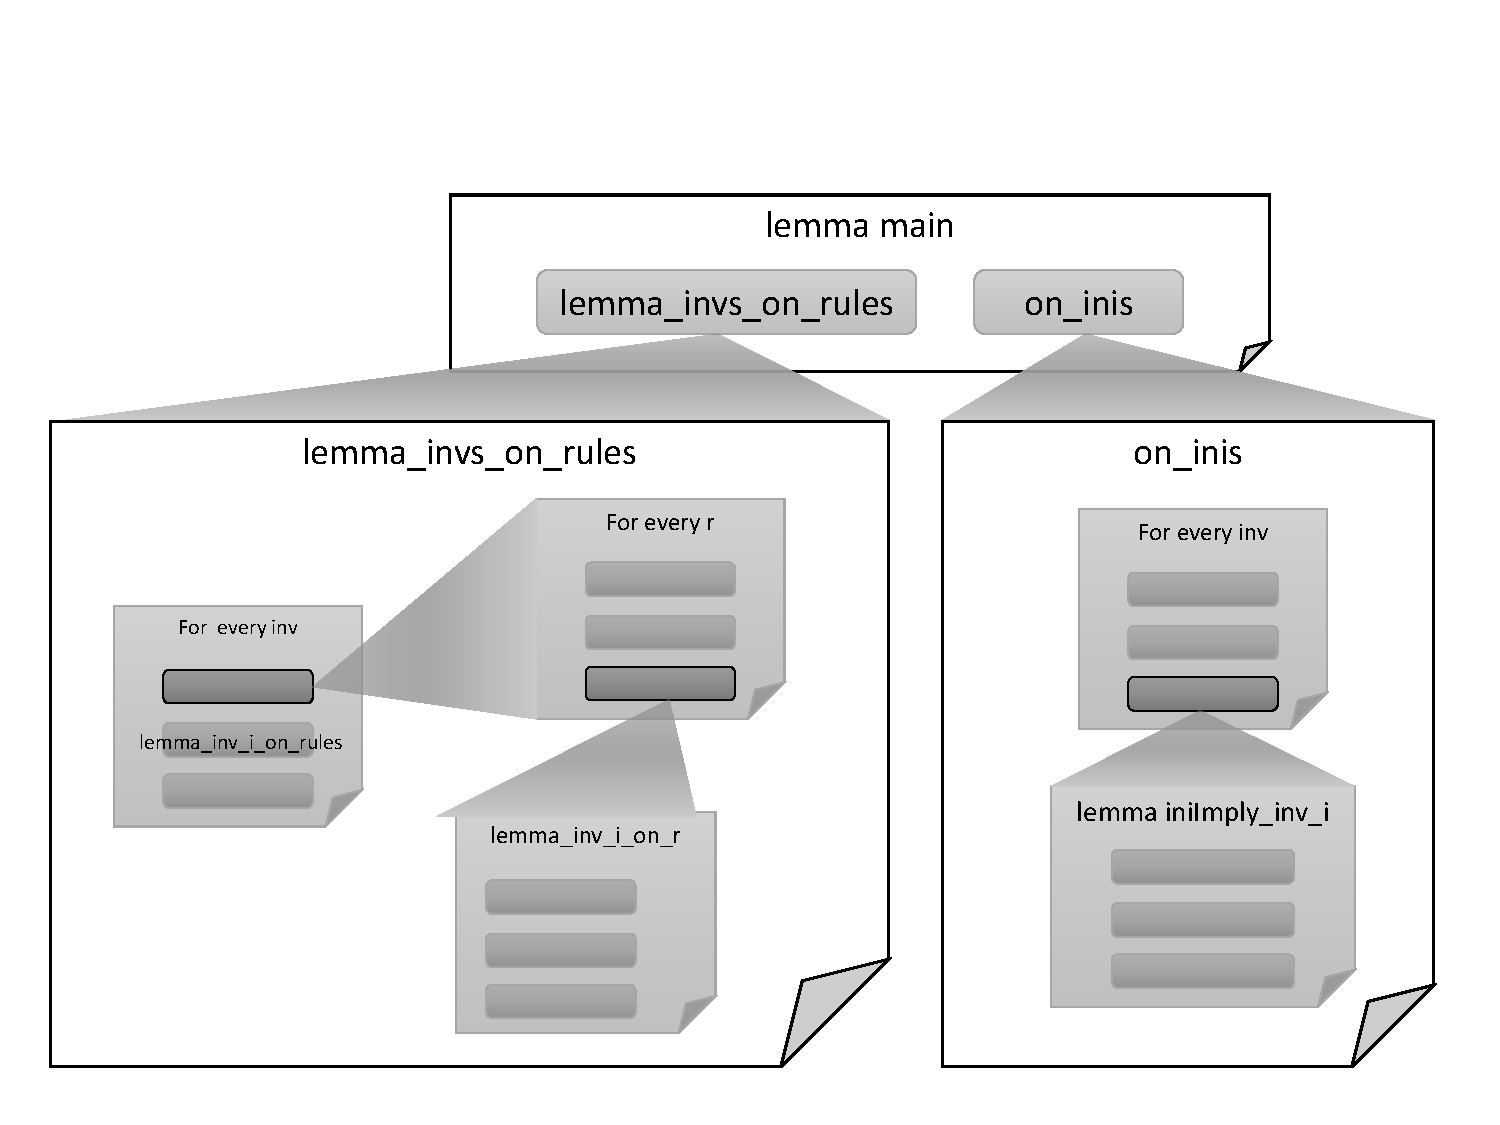
\includegraphics[width=1.0\textwidth]{thy.pdf}
%\vspace{-0.5cm}
 \caption{The hierachy of lemmas}

\end{figure}

 % Now we discuss how to use records on {\tt crit} and {\tt inv$_1$} in the tables   $symbInvs$, $symbRules$, and $symbCausalTab$ to generate a lemma to prove that causal relation hold between   crit and   $inv_1$, which will be applied in the proof of main lemma.
\subsubsection{Lemmas for Causal Relation between Rules and Invariants}
 A lemma at the bottom level, specifies that causal relation hold between  a rule like  {\tt crit} and a parameterized rule like  $inv_1$, An  example lemma
{\tt critVsinv$_1$} and its proof in Isabelle in the {\tt mutualEx} protocol, is illustrated as follows:


\begin{specification}
%\begin{algorithm}
%\caption{Generating a kind of proof which is according with a relation tag of $invHoldForRule_{1-3}$ : rel2proof}\label{lemma:causal relation lemma}
1lemma critVsinv1:\\
2  assumes  a1: $\exists$ \iR1. \iR1 $\le$ N $\wedge$ r=crit \iR1 and \\
  a2: $\exists$  \iInv1 \iInv2. \iInv1 $\le$ N $\wedge$ \iInv2 $\le$ N $\wedge$ \iInv1 $\neq$ \iInv2 $\wedge$ f=inv1  \iInv1 \iInv2\\
3  shows  invHoldForRule s f r (invariants
  N)\\
4  proof -\\
   from a1 obtain \iR1 where a1:\iR1 $\le$ N $\wedge$ r=crit \iR1 \\
\twoSpaces   by blast\\
   from a2 obtain \iInv1 \iInv2 where \\
   a2: \iInv1 $\le$ N $\wedge$ \iInv2 $\le$ N $\wedge$ \iInv1 $\neq$ \iInv2 $\wedge$ f=inv1  \iInv1 \iInv2\\
\twoSpaces   by blast \\
5  have iR1=\iInv1 $\vee$ \iR1=\iInv2 $\vee$ (\iR1 $\ne$ \iInv1 $\wedge$  \iR1 $\ne$ \iInv2) by auto\\

6  moreover\{assume  b1:\iR1=\iInv1\\
7  \twoSpaces have invHoldForRule3 s f r (invariants N)\\
 \twoSpaces  \twoSpaces   proof(cut\_tac a1 a2 b1, simp, rule\_tac x=$\negc$ (x=true $\andc$ n[\iInv2]=C)  in exI,auto)qed\\
8  \twoSpaces then have invHoldForRule s f r
(invariants
  N)
by auto\}\\

9  moreover\{assume  b1:iR1=\iInv2\\
10 \twoSpaces have invHoldForRule3 s f r (invariants N)\\
 \twoSpaces \twoSpaces   proof(cut\_tac a1 a2 b1, simp, rule\_tac x=$\negc$ (x=true $\andc$ n[\iInv1]=C  in exI,auto)qed\\
11 \twoSpaces then have invHoldForRule s f r (invariants
  N)
by auto\}\\

12   moreover\{assume  b1:(\iR1 $\ne$  \iInv1 $\wedge$   \iR1 $\ne$  \iInv2)\\
13 \twoSpaces have invHoldForRule2 s f r  \\
  \twoSpaces \twoSpaces  proof(cut\_tac a1 a2 b1,  auto) qed\\
14 \twoSpaces then have invHoldForRule s f r
(invariants
  N)
by auto\} \\

15ultimately show invHoldForRule s f r
(invariants N) by blast\\
16qed\\
%\end{algorithm}
\end{specification}

A lemma such as {\tt critVsinv1}  is generated by collecting all the records on the invariant {\tt inv1} and rule {\tt crit} in the aforementioned tables.
Line 2 are assumptions on the parameters of the invariant and rule, which are composed of two parts: (1) assumption {\tt a1} specifies that there exists an actual parameter {\tt \iR1} with which {\tt r} is a rule obtained by instantiating {\tt crit}; (2) assumption {\tt a2} specifies that  there exists   actual parameters {\tt \iInv1} and {\tt \iInv2} with which {\tt f} is a formula obtained by instantiating {\tt inv1}.
 %(1) the facts that all parameters of this invariant should be less than the parameter $N$; %(2) the facts that all parameters of this invariant should be less than the parameter $N$; (3) the constraints of he mutual difference between parameters of the invariant (rule), which can %be looked up in the field of those records  from the table $symbInvTab$ ($symbRuleTab$) by the invariant (rule) name {\tt inv1} ({\tt crit}), which specifies that the mutual difference %between two parameters.
Line 4 are two typical  proof patterns forward-style which fixes local variables such as {\tt \iR1} and new facts such as {\tt a1: iR1 $\le$ N $\wedge$ r=crit \iR1}. From line 5, the remaining parts of the proof is a typically readable one in Isar style \cite{Wen99}, which uses calculation
reasoning such as {\tt moreover} and {\tt ultimately} to do  case analysis.
Line 5 splits cases of {\tt iR1} into all possible cases by comparing
{\tt \iR1} with {\tt \iInv1} and {\tt \iInv2}, which is in fact characterized by $partition([1],[2],[3]],[1,2])$. Lines 6-14  proves    these cases one by one: Lines 6-8 proves the case where {\tt iR1=\iInv1}, line 7 first proves that the causal relation $invHoldForRule_3$ holds by supplying a formula, which is $symbolize'(invOnXC(2),[1,2],[1])$. %Notes that $invOnXC(2)$ is the $f'$ which is provided in the last column of the line.
From the conclusion at line 7, line 8 futhermore proves the causal relation $invHoldForRule$ hold; Lines 9-11 proves the case where {\tt iR1=\iInv2}, proof of which is similar to that of case 1; Lines 12-14 the case   where neither {\tt iR1=\iInv1} nor {\tt iR1=\iInv2}. Each proof of a subcase is done in a block {\tt moreover b1:asm1 proof1}, the {\tt ultimately}  proof command in line 15 concludes by summing up all the subcases.




With the help of all the lemmas such as {\sf ruleVsinv1},  we can prove the following lemma  {\sf lemma$\_$inv$\_$1$\_$on$\_$rules} which
specifies that for all $r \in rules ~N$, and $f$ is a formula $f$ which is generated by instantiating inv1 with some parameters $\iInv_1$ and $iInv_2$, $invHoldForRule ~s~ f~ r~ (invariants~ N)$.

\begin{specification}
lemma lemma$\_$inv1$\_$on$\_$rules:
  $\isasymlbrakk$ a1:
r $\in$ rules N
 and a2:
($\exists$ $\_$iInv1 $\_$iInv2. $\_$iInv1$\le$
N$\wedge$$\_$iInv2$\le$\\
N$\wedge$\iInv1$\neq$\iInv2$\wedge$f=inv1  \iInv1 \iInv2)\\

  $\isasymrbrakk\Longrightarrow$
invHoldForRule s f r (invariants N)\\

  proof -\\
\twoSpaces  have
($\exists$ i. i$\le$
N$\wedge$r=try  i)$\vee$
    ($\exists$ i. i$\le$\\
N$\wedge$r=crit  i)$\vee$
    ($\exists$ i. i$\le$
N$\wedge$r=exit  i)$\vee$\\
    ($\exists$ i. i$\le$
N$\wedge$r=idle  i)\\

  apply (cut$\_$tac a1, auto) done\\
    moreover $\{$      assume b1:
($\exists$ i. i$\le$
N$\wedge$r=try  i)\\

\twoSpaces      have invHoldForRule' s f r (invariants N)\\

\twoSpaces      apply (cut$\_$tac a2 b1, metis tryVsinv1) done
    $\}$\\


    moreover $\{$ assume a1:
($\exists$ i. i$\le$
N$\wedge$r=crit  i)\\

\twoSpaces      have
invHoldForRule' s f r (invariants N)\\

\twoSpaces      apply (cut$\_$tac a2 b1, metis critVsinv1) done
    $\}$\\


    moreover $\{$
      assume a1:
($\exists$ i. i$\le$
N$\wedge$r=exit  i)\\

\twoSpaces      have
invHoldForRule' s f r (invariants N)\\

\twoSpaces      apply (cut$\_$tac a2 b1, metis exitVsinv1) done
    $\}$\\


    moreover $\{$ assume a1:
($\exists$ i. i$\le$
N$\wedge$r=idle  i)\\

\twoSpaces      have
invHoldForRule' s f r (invariants N)\\

\twoSpaces      apply (cut$\_$tac a2 b1, metis idleVsinv1) done
    $\}$\\


  ultimately show invHoldForRule' s f r (invariants N)\\
  by auto\\
qed\\

\end{specification}

With the help of all the lemmas such as {\sf lemma$\_$inv$_i\_$on$\_$rules},  we can prove the following lemma  {\sf invs$\_$on$\_$rules} which
specifies that for all $f \in invariants~ N$ and $r \in rules~ N$,   $invHoldForRule ~s~ f~ r~ (invariants~ N)$.

\begin{specification}
lemma invs$\_$on$\_$rules:
  $\isasymlbrakk$ a1:
f $\in$ invariants N
 and a2:
r $\in$ rules N
  $\isasymrbrakk\Longrightarrow$\\
invHoldForRule' s f r (invariants N)\\

  proof -\\
  have b1:
($\exists$ \iInv1 \iInv2. \iInv1$\le$
N$\wedge$\iInv2$\le$
N$\wedge$\iInv1$\neq$\iInv2$\wedge$f=inv1  \iInv1 \iInv2)$\vee$\\
    ($\exists$ \iInv2. \iInv2$\le$
N$\wedge$f=inv2  \iInv2)$\vee$\\
    ($\exists$ \iInv1 \iInv2. \iInv1$\le$
N$\wedge$\iInv2$\le$
N$\wedge$\iInv1$\neq$\iInv2$\wedge$f=inv3  \iInv1 \iInv2)$\vee$\\
    ($\exists$ \iInv2. \iInv2$\le$
N$\wedge$f=inv4  \iInv2)$\vee$\\
    ($\exists$ \iInv1 \iInv2. \iInv1$\le$
N$\wedge$\iInv2$\le$
N$\wedge$\iInv1$\neq$\iInv2$\wedge$f=inv5  \iInv1 \iInv2)\\

  apply (cut$\_$tac a1, auto) done\\
    moreover $\{$      assume b1:
($\exists$ \iInv1 \iInv2. \iInv1$\le$
N$\wedge$\iInv2$\le$
N$\wedge$\iInv1$\neq$\iInv2$\wedge$f=inv1  \iInv1 \iInv2)\\

\twoSpaces       have
invHoldForRule' s f r (invariants N)\\

\twoSpaces      apply (cut$\_$tac a2 b1, metis lemma$\_$inv1$\_$on$\_$rules) done
    $\}$\\


    moreover $\{$ assume b1:
($\exists$ \iInv2. \iInv2$\le$
N$\wedge$f=inv2  \iInv2)\\

\twoSpaces       have invHoldForRule' s f r (invariants N)\\

\twoSpaces      apply (cut$\_$tac a2 b1, metis lemma$\_$inv2$\_$on$\_$rules) done
    $\}$\\


    moreover $\{$      assume b1:
($\exists$ \iInv1 \iInv2. \iInv1$\le$
N$\wedge$\iInv2$\le$
N$\wedge$\iInv1$\neq$\iInv2$\wedge$f=inv3  \iInv1 \iInv2)\\

\twoSpaces       have
invHoldForRule' s f r (invariants N)\\

\twoSpaces      apply (cut$\_$tac a2 b1, metis lemma$\_$inv3$\_$on$\_$rules) done
    $\}$\\


    moreover $\{$      assume b1:
($\exists$ \iInv2. \iInv2$\le$
N$\wedge$f=inv4  \iInv2)\\

\twoSpaces       have
invHoldForRule' s f r (invariants N)\\

\twoSpaces      apply (cut$\_$tac a2 b1, metis lemma$\_$inv4$\_$on$\_$rules) done
    $\}$\\


    moreover $\{$
      assume b1:
($\exists$ \iInv1 \iInv2. \iInv1$\le$
N$\wedge$\iInv2$\le$
N$\wedge$\iInv1$\neq$\iInv2$\wedge$f=inv5  \iInv1 \iInv2)\\

\twoSpaces       have
invHoldForRule' s f r (invariants N)\\

\twoSpaces      apply (cut$\_$tac a2 b1, metis lemma$\_$inv5$\_$on$\_$rules) done
    $\}$\\


  ultimately show
invHoldForRule' s f r (invariants N)\\

\twoSpaces  apply fastforce done\\
qed
end\\
\end{specification}



 % {\tt allSymbRecs } are all symbolic causal relation records on {\tt  invName} and {\tt  ruleName},
% then  {\tt lenPInv} and {\tt lenPRule} which are numbers of the parameters of the invariant formula and rule, then {\tt asms} which are the assumptions part of the lemma such as line 2, {\tt allDisjuncts} the case analysis between the parameters of invariant and rule such as line 5, {\tt allSubProofs} all the proofs of the subcases such as lines 6-14, then fill all these into the blanks of the templates to generate the lemma.


% {\tt namedAsmTrans asm i} adds a name "ai:" to a string of assumption in order to construct a named assumption. {\tt allNamedAsmsGen} generates all the aformentioned  four kinds of assumptions of the lemma in the previous paragrapgh: {\tt asmsLessOnInv} is according with (1) types of assumptions; {\tt asmsLessOnRule} (2) types of assumptions;  {\tt asmsMutualDiffOnInv} (3) types of assumptions; and {\tt asmsMutualDiffOnRule} (4) types of assumptions. After naming any one assumption with a name, {\tt allNamedAsmsGen} returns all the named assumptions which are conned by {\tt and} operator. {\tt symbCausalRec2Proof symbRec} generates a kind of proof in Isabelle according to a symbolic casual relation record {\tt symbRec}: if the tag of {\tt holdTag} is 1(2,3), then kind 1 (2,3) proof are generated accordingly. Here we list the most complex one: {\tt proof3Gen ruleName invName f}, which generates a proof which is according with {\tt invHoldType3} such as lines 6-8, and {\tt f} is another invariant formula which is needed to construct the {\tt invHoldType3} causal relation.
%\twoSpaces  let asmsLessOnRule=asmsGen iRule sN lenPRule in \\
%\twoSpaces  let asmsMutualDiffOnInv=asmsLookUp symbInvs invName gFldName in\\
%\twoSpaces  let asmsMutualDiffOnRule
\subsubsection{Lemmas on initial states}

In this section, we discuss the definition on the initial state of the protocol, and the lemmas specifying that each invariant formula holds at the initial state.

A typical Isabelle definition on the initial state of the protocol is as follows:

\begin{specification}
definition initSpec0::nat $\Rightarrow$ formula where [simp]:\\
initSpec0 N $\equiv$ (forallForm (down N) (\% i . (eqn (IVar (Para (Ident ''n'') i)) (Const I))))\\

definition initSpec1::formula where [simp]:\\
initSpec1  $\equiv$ (eqn (IVar (Ident ''x'')) (Const true))\\

definition allInitSpecs::nat \<Rightarrow> formula list where [simp]:\\
allInitSpecs N $\equiv$ [(initSpec0 N),(initSpec1 )]\\

lemma iniImply\_inv4:
assumes a1: ($\exists$\iInv1. \iInv1$\le$N$\wedge$f=inv4 \iInv1)\\
and a2: formEval (andList (allInitSpecs N)) s\\
shows formEval f s\\
 using a1 a2 by auto\\
\end{specification}

{\tt initSpec0} and {\tt initSpec1} specifies the assignments on each variable {\tt n[i]} where {\tt i $\le$ N} and {\tt x}. The  specifications of the initial state is the list of all the specification definition on related state variables. Lemma {\tt iniImply\_inv4} simply specifies that the invariant formula {\tt inv4} holds at a state {\tt s} which satisfies the conjunction of the   specification of the initial state. Isabelle's {\tt auto} method can solve this goal automatically. Other lemmas specifying that other invariant formulas hold at the initial state are similar.
%The generation of the above code is straightforward: definitions of the specification of initial state variables in Isabelle is a direct syntax transformation from the internal represetation of tool {\tt proofGen} to Isabelle.

With the lemmas such as {\tt iniImply\_inv4}, for any invariant $inv \in (\mathsf{invariants} ~N) $,  any
state $s$, if $ini$ is evaluated true at state $s$, then $inv$ is
evaluated true at state $s$.

\begin{specification}
lemma on$\_$inis:
  $\isasymlbrakk$ a1:
f $\in$ (invariants N)
 and a2:
ini $\in$ $\{$
andList (allInitSpecs N)$\}$\\

 and a3:
formEval ini s

  $\isasymrbrakk\Longrightarrow$
formEval f s\\

  proof -\\
  have c1:
($\exists$ \iInv1 \iInv2. \iInv1$\le$
N$\wedge$\iInv2$\le$
N$\wedge$\iInv1$\neq$\iInv2$\wedge$f=inv$\_$$\_$1  \iInv1 \iInv2)$\vee$\\
    ($\exists$ \iInv2. \iInv2$\le$
N$\wedge$f=inv$\_$$\_$2  \iInv2)$\vee$\\
    ($\exists$ \iInv1 \iInv2. \iInv1$\le$
N$\wedge$\iInv2$\le$
N$\wedge$\iInv1$\neq$\iInv2$\wedge$f=inv$\_$$\_$3  \iInv1 \iInv2)$\vee$\\
    ($\exists$ \iInv2. \iInv2$\le$
N$\wedge$f=inv$\_$$\_$4  \iInv2)$\vee$\\
    ($\exists$ \iInv1 \iInv2. \iInv1$\le$
N$\wedge$\iInv2$\le$
N$\wedge$\iInv1$\neq$\iInv2$\wedge$f=inv$\_$$\_$5  \iInv1 \iInv2)\\

\twoSpaces  apply (cut$\_$tac a1, simp) done\\
    moreover $\{$
      assume b1:
($\exists$ \iInv1 \iInv2. \iInv1$\le$
N$\wedge$\iInv2$\le$
N$\wedge$\iInv1$\neq$\iInv2$\wedge$f=inv$\_$$\_$1  \iInv1 \iInv2)\\

      have
formEval f s\\

\twoSpaces      apply (rule iniImply$\_$inv$\_$$\_$1)\\
\twoSpaces      apply (cut$\_$tac b1, assumption)\\
\twoSpaces      apply (cut$\_$tac a2 a3, blast) done
    $\}$\\


    moreover $\{$
      assume b1:
($\exists$ \iInv2. \iInv2$\le$
N$\wedge$f=inv$\_$$\_$2  \iInv2)\\

      have
formEval f s\\

\twoSpaces      apply (rule iniImply$\_$inv$\_$$\_$2)\\
\twoSpaces      apply (cut$\_$tac b1, assumption)\\
\twoSpaces      apply (cut$\_$tac a2 a3, blast) done\\
    $\}$\\


    moreover $\{$
      assume b1:
($\exists$ \iInv1 \iInv2. \iInv1$\le$
N$\wedge$\iInv2$\le$
N$\wedge$\iInv1$\neq$\iInv2$\wedge$f=inv$\_$$\_$3  \iInv1 \iInv2)\\

      have
formEval f s\\

\twoSpaces      apply (rule iniImply$\_$inv$\_$$\_$3)\\
\twoSpaces      apply (cut$\_$tac b1, assumption)\\
\twoSpaces      apply (cut$\_$tac a2 a3, blast) done
    $\}$\\


    moreover $\{$
      assume b1:
($\exists$ \iInv2. \iInv2$\le$
N$\wedge$f=inv$\_$$\_$4  \iInv2)\\

      have
formEval f s\\

\twoSpaces      apply (rule iniImply$\_$inv$\_$$\_$4)\\
\twoSpaces      apply (cut$\_$tac b1, assumption)\\
\twoSpaces      apply (cut$\_$tac a2 a3, blast) done
    $\}$\\


    moreover $\{$
      assume b1:
($\exists$ \iInv1 \iInv2. \iInv1$\le$
N$\wedge$\iInv2$\le$
N$\wedge$\iInv1$\neq$\iInv2$\wedge$f=inv$\_$$\_$5  \iInv1 \iInv2)\\

      have
formEval f s\\

\twoSpaces      apply (rule iniImply$\_$inv$\_$$\_$5)\\
\twoSpaces      apply (cut$\_$tac b1, assumption)\\
\twoSpaces      apply (cut$\_$tac a2 a3, blast) done
    $\}$\\


  ultimately show formEval f s
  by auto\\
qed\\


\end{specification}

The proof structure of {\sf lemma$\_$inv1$\_$on$\_$rules} and  {\sf invs$\_$on$\_$rules} and {\sf on$\_$inis} are also typical case analysis ones using {\sf moreover} blocks and {\sf ultimately} commands, therefore, a generic program of generating a typical case analysis proof will be adopted in our framework.

%All can be generated by calling the generic template function {\sf doCaseAnalz} with different subproof generation functions.


\subsubsection{The main theorem}

%-------------------------------------------------------------------------
%At last, we discuss how to create automatically the proof for the main lemma, which depends
% on the applying the lemmas which are created in subsection \ref{sec:genOfIsabelleProof}.
With the preparation of lemma  on$\_$inis and  invs$\_$on$\_$rules, the generation of the main lemma is quite easy. Recall that the consistency lemma is our
main weapon to prove the main lemma, which requires proving two parts of
obligations.



\begin{description}
\item[(1)] For any invariant $inv \in (\mathsf{invariants} ~N) $,  any
state $s$, if $ini$ is evaluated true at state $s$, then $inv$ is
evaluated true at state $s$. This can be solved done by applying lemma on$\_$inis.
\item[(2)]  For any invariant $inv \in (\mathsf{invariants} ~N)$, any $r$ in rule set
$ \mathsf{rules} ~N$ , one of the causal relations
$\mathsf{invHoldForRule}_{1-3}$ holds. This can be solved done by  applying lemma invs$\_$on$\_$rules.
\end{description}
%
%Proof of Part (1) is  simple. %%For an invariant
%$inv=\mathsf{implyForm}~ant~cons$ in $invs$, we only need to prove
%that either $ant$ is evaluated as false or $cons$ is evaluated true
%at an initial state $s$ in order to prove $\models
%~inv~s$. Such a proof  can be automatically solved by Isabelle's
%$\mathsf{auto}$ command.



\begin{specification}
lemma main:
  $\isasymlbrakk$  s$\in$ reachableSet \{andList (allInitSpecs N)\} (rules N); 0<N$\isasymrbrakk$\\
  $\Longrightarrow$ $\forall$ inv. inv $\in$ (invariants N) $\longrightarrow$ formEval inv s\\
proof(rule consistentLemma)\\
  show consistent (invariants N) \{andList (allInitSpecs N)\} (rules N)\\
 proof(cut\_tac a1, unfold consistent\_def,rule conjI)\\
   show  $\forall$inv ini s. inv $\in$ (invariants N)
$\longrightarrow$ ini $\in$\{andList (allInitSpecs N)\}$\longrightarrow$formEval
ini s $\longrightarrow$ formEval inv s\\
proof((rule allI)+,(rule impI)+)\\
\twoSpaces   fix inv ini s\\
\twoSpaces   assume b1:inv $\in$ (invariants N) \\
\twoSpaces     and b2:ini $\in$ \{andList (allInitSpecs N)\}  and b3:formEval ini s\\
\twoSpaces   show "formEval f s"\\
\twoSpaces   apply (rule on\_inis, cut\_tac b1, assumption, cut\_tac b2, assumption, cut\_tac b3, assumption) done\\
    qed\\

next   show  $\forall$inv r. inv $\in$ invariants N$\longrightarrow$
 r $\in$rules N$\longrightarrow$invHoldForRule inv r (invariants N) \\

   proof((rule allI)+,(rule impI)+)\\
\twoSpaces      fix f r \\
\twoSpaces         assume b1: f $\in$ invariants N  and b2:r $\in$ rules N\\

\twoSpaces     show "invHoldForRule' s f r (invariants N)"\\
  apply (rule invs\_on\_rules, cut\_tac b1, assumption, cut\_tac b2, assumption) done\\
qed\\
next show "s $\in$ reachableSet {andList (allInitSpecs N)} (rules N)"
  apply (metis a1) done\\
qed\\
\end{specification}

The generation of the main lemma is quite easy because it is in a standard form.
%\vspace{-0.5cm}
 %in order to verify the cache coherence protocols. Others are straightforward.
%The proof is a typically
%readable one in Isar style \cite{}, which uses calculation
%reasoning such as {\tt moreover} and {\tt ultimately} to do  case analysis on
%the form of rules and the invariants. Lines 1-5 use proper Isabelle
%proof commands to   decompose the main proof goal of forall  and
%implication form,    fix a rule {\tt r} and {\tt inv}, then have two
%assumptions {\tt  b1: inv$\in$ invariants N  and b2:r $\in$ rules
%N}, now we need show the goal {\tt invHoldForRule s f r (invariants
%N)}. line 5 splits cases of $r$ into all possible cases according to
%the definition of $rules~N$. %In order to save space, we adopt the following abbreaviation:
% $\mathsf{ex1P}~ N~ P \equiv \exists i. (i \le N \wedge P~
%i)$, $\mathsf{ex2P}~ N~ P \equiv \exists i~j. (i \le N \wedge j \le
%N \wedge i\ne j \wedge P~ i~j)$, and $\mathsf{ex3P}~ N~ P \equiv
%\exists i~j~k. (i \le N \wedge j \le N \wedge k \le N\wedge i\ne j
%\wedge i\ne k \wedge j\ne k \wedge P~ i~j~k)$.
%Line 6 starts the case analysis on
%$r=r_0$. Line 7 again splits cases of $inv$ into all possible cases
%according to the definition of $invariants~N$. Line 8-10 proves the
%goal at case when $r=exit$ and $inv=inv1$. At line 10,  a  proved
%lemma {\tt exitVsInv1}  is directly applied to solve the proof
%goal.  Similiarly, we can do subproofs on other cases on {\tt inv},
%and finish the proof goal accordingly.
% After finishing the proof of the last case  of $inv=inv5$,
% we finish the proof of the first case $r=exit$. Similarly, we can
% finish the proof goal at
%each subcase on {\tt r}. At  lines 19 and  20 we show we have
%finished the proof goal formally.

\subsection{Algorithms of Proof Generator {\sf proofGen}}

In this subsection, we illustrate the key techniques and algorithms of generation of the lemmas and their proofs in subsection \ref{subsection:introOfIsabelleProof}. Being according with the order in which we introduce the above lemmas, we also introduce their generation in a bottom-up order. First let us introduce the generation of a subproof according to a relation tag of $invHoldForRule_{1-3}$, which is shown in Algorithm \ref{alg:proofGenOfReltag}.

\begin{algorithm}
\caption{Generating a kind of proof which is according with a relation tag of $invHoldForRule_{1-3}$ : rel2proof}\label{alg:proofGenOfReltag}
\KwIn{A causal    relation item $relTag$}
\KwOut{  An Isablle proof: $proof$   }

{
 \If{$relTag=invHoldForRule_1$}
  {$proof \leftarrow $ sprintf\\
\twoSpaces"have invHoldForRule1 f r (invariants N)  \\
\twoSpaces         by(cut\_tac a1 a2 b1, simp, auto) \\
\twoSpaces then have invHoldForRule f r (invariants N)  by blast" \; }
 \ElseIf{ $relTag=invHoldForRule_2$}
  {$proof \leftarrow$  sprintf\\
\twoSpaces"have invHoldForRule2 f r (invariants N)
\twoSpaces         by(cut\_tac a1 a2 b1, simp, auto) \\
\twoSpaces then have invHoldForRule f r (invariants N)  by blast" \; }
 \Else{
 \label{label:getFormField}$f' \leftarrow getFormField(relTag)$\;
 $proof \leftarrow$ sprintf\\
\twoSpaces"have invHoldForRule3 f r (invariants N)  \\
\twoSpaces proof(cut\_tac a1 a2 b1, simp, rule\_tac x=\%s  in exI,auto)qed\\
\twoSpaces then have invHoldForRule f r (invariants N)  by blast" (symbf2Isabelle f')"\;}
\Return{proof}
}
\end{algorithm}

In the body of function {\sf rel2proof},  $sprintf$ writes a formatted data to string and returns it.
In line \ref{label:getFormField}, $getFormField(relTag)$ returns $f'$ if $relTag=invHoldForRule_3(f')$.  {\sf rel2proof} transforms a a relation tag into a paragraph of proof.% as shown in lines 7-8, 10-11, or 13-14.
If the tag is among $invHoldForRule_{1-2}$, the transformation is rather straight-forward, else the form $f'$ is assigned by the formula $getFormField(relTag)$, and provided to tell Isabelle the formula which should be used to construct the $invHoldForRule_3$ relation.

\begin{algorithm}
\caption{Generating one sub-proof for a subcase: oneMoreOverGen}\label{alg:MoreOver}

\KwIn{A formula $caseFsm$ standing for the assumption of the subcase, a relation item $relItem$ containing the information of causal relation }
\KwOut{  An Isablle proof: $subProof$ }
{
%$label \leftarrow labelGen(depth) $\;
$proof \leftarrow rel2proof(relItem)$\;
$  subProof \leftarrow$  sprintf\\
%\twoSpaces sprintf\\
\twoSpaces "moreover\{assume  b1:\%s  \\
           \%s    \} "\\
\twoSpaces ( asm, proof)\;
\Return{subproof}
}
\end{algorithm}

In Algorithm \ref{alg:MoreOver}, {\sf oneMoreOverGen} generates a subproof for a subcase in a proof of case analysis. It returns a subproof which is composed by filling an assumption of the subcase such as "\iR1=\iInv1" and a paragraph of proof generated by $rel2proof(relItem)$ into a format of block {\tt morover \{ ...\}}.  %the input $depth$ shows the  the depth of the current proof. Recalling that proof is recursively composed by subproofs. Each level of proofs are tagged with some depth. {\sf labelGen(depth)} returns a label such as $a1:$. {\sf oneMoreOverGen} generates a subproof which is

Due to the common use of case analysis proof of using {\sf moreover} and {\sf ultimately} commands, we design a generic program of generating  doing case analysis {\sf doCaseAnalz}. In algorithm \ref{alg:doCaseAnalz}, %generates a typical proof of doing case analyis.
 formulas standing for case-splitting $partition$, subproofs $subproofs$, and the conclusion $concluding$ are needed  in case analysis to fill the format.
\begin{algorithm}

\caption{Generating a whole proof of doing case analysis: doCaseAnalz}\label{alg:doCaseAnalz}
\KwIn{A formula $partition$ standing for case-splittings, a proof list $subproofs$ standing  all the subproofs of each subcases, concluding parts $concluding$}%, the depth of proof $depth$ }
\KwOut{  An Isablle proof: $proof$ }
{

%\If{$depth=1$}
%{$showOrHave \leftarrow$ "show"\;}
%\Else {$showOrHave \leftarrow$ "have"\;}
$proof \leftarrow $sprintf\\
\twoSpaces \twoSpaces  " have \%s  by auto\\
\twoSpaces \twoSpaces         \%s\\
\twoSpaces \twoSpaces        ultimately show \%s by auto"\\
\twoSpaces     (partition, subproofs,  concluding) \;
\Return{proof}
}
\end{algorithm}


In algorithm \ref{alg:doCaseAnalzI}, {\sf caseAnalzI} generates a typical proof of doing case analysis to  prove some causal relation hold between some rule and invariant. oneMoreOverGenI(case,rel) formula comes from the disjunction of formulas in the {\tt symbCases} field of $rec$, which is returned by $caseField(rec)$, subproofs $subproofs$ are generated by concatenation of all the subproofs, each of which is generated by $oneMoreOverGenI(case,rel)$. The proof is simply composed by  calling $doCaseAnalz(partition,subproofs,concluding)$.

\begin{algorithm}

\caption{Generating a whole proof of doing case analysis on parameters of rule and invariant: caseAnalzI}\label{alg:doCaseAnalzI}
\KwIn{A record $rec$ fetched from $symbCausal$ }
\KwOut{  An Isablle proof: $proof$ }
{
$cases \leftarrow caseField(rec)$\;
$rels \leftarrow relItems(rec)$;
$partition \leftarrow \bigvee cases$\;
$subproofs \leftarrow ""$\;
\While{$(cases \ne [])$}
{ $ case \leftarrow hd(cases)$ \;
  $cases \leftarrow tl(cases)$ \;
  $ rel \leftarrow hd(rels)$ \;
  $rels \leftarrow tl(rels)$ \;
  $subproofs \leftarrow subproofs \cat oneMoreOverGenI(case,rel)$\;
  }
$ concluding \leftarrow $"invHoldForRule s f r (invariants N) "\;
$proof \leftarrow doCaseAnalz(partition,subproofs,concluding)$\;
\Return $proof$
}
\end{algorithm}

Next we discuss how to generate assumptions on an invariant formula of an lemma such as $critVsInv1$. In the body of algorithm \ref{alg:asmGenOnInv}, $tbl\_element(symbInvs,  invName)$  retrieves the record on a invariant formula from $symbInvs$ to $invItem$ by its name $invName$, $invParaNum(invItem  )$ and $constrOfInv(invItem))$ return the field {\tt invNumFld} and {\tt constr} of  $invItem$ respectively. $invParasGen(lenPInv)$ generates a string of a list of actual parameters such as $iInv_1 ... iInv_{lenPInv}$ if $lenPInv>0$, else an empty string "".  At last, the assumption on the invariant is created by filling $invParas$,  $constrOnInv$, and $invName$ into a proper place in the format if needed.

\begin{algorithm}
  \caption{Generating an assumption on an invariant formula: asmGenOnInv}\label{alg:asmGenOnInv}
  \KwIn{An invariant name $invName$,    a table $symInvs$ storing invariant formulas   }

\KwOut{  An assumption on an invariant formula: $asm$   }

 $invItem   \leftarrow tbl\_element( symbInvs,  invName)$\;
  $lenPInv \leftarrow invParaNum(invItem  )$\;
  $invParas \leftarrow invParasGen(lenPInv)$\;
 % $constrOfInv \leftarrow constr(N,lenPInv)$\;
 $constrOnInv \leftarrow symbForm2Isabelle(constrOfInv(invItem))  $\;
 \If {lenPInv = 0}
  {$asm  \leftarrow  "a1: f="\cat invName   $\;}
  \Else{$asm  \leftarrow$ sprintf "a1: $\exists$ \%s. \%s $\wedge$ f=\%s \%s" (invParas,  constrOnInv, invName, invParas)\;}
  \Return{asm}
\end{algorithm}

Similar to {\sf asmGenOnInv}, {\sf obtainGenOnInv}, which is shown in algorithm \ref{alg:obtainGenOnInv}, generates a proof command of {\sf obtain} by retrieving and generating the related information and filling them in a format on {\sf obtain}.  Similar to {\sf asmGenOnInv} and  {\sf obtainGenOnInv}, {\sf asmGenOnRule} and  {\sf obtainGenOnRule} generate an  assumption and {\sf obtain} proof command   on a rule.

\begin{algorithm}
  \caption{Generating an {\sf obtain} proof command on an invariant formula: obtainGenOnInv}\label{alg:obtainGenOnInv}
  \KwIn{An invariant name $invName$,    a table $symInvs$ storing rules    }
  $invItem   \leftarrow tbl\_element( symbInvs,  invName)$\;
  $lenPInv \leftarrow invParaNum(invItem  )$\;
  $invParas \leftarrow invParasGen(lenPInv)$\;
\If {$  lenPInv = 0 $}
    {$obtain \leftarrow  ""$\;}
 \Else {$obtain \leftarrow$ sprintf "from a1 obtain  \%s where a1:\%s $\wedge$ f=\%s \%s by auto"\\
 \twoSpaces           $(invParas,  constrOnInv, invName, invParas)$\;}
 \Return{obtain}
\end{algorithm}



After the above preparing functions, now the generation of a lemma on the causal relation such as    $critVsInv1$ is rather easy, which is shown in algorithm \ref{alg:lemmaOnCausalRuleInv}. After generating an assumption on invariant formula $asm1$,  $asm2$ on a rule, an obtain command  $obtain1$ on the invariant, and  $obtain2$ on the rule,  $symRelItem$ is retrieved from $symCausalTab$ by $ruleName\cat invName$, and a proof $proof$ is generated by calling $caseAnalzI(symRelItem)$. At last these parts are filled into proper places in the lemma format.

\begin{algorithm}
\caption{Generating a lemma on a causal relation: lemmaOnCausalRuleInv}\label{alg:lemmaOnCausalRuleInv}

\KwIn{A parameterized rule name $ruleName$,   a formula name $invName$, a table $symRules$ storing rules , a table $symInvs$ storing invariant formulas,   a table $symCausalTab$  storing causal relation  }

\KwOut{  An Isablle proof script for a lemma: $lemmaWithProof$   }

{


 $asm1 \leftarrow asmGenOnInv(symbInvs,invName)$\;
 $asm2 \leftarrow asmGenOnRule(symbRules,ruleName)$\;
 $obtain1 \leftarrow obtainGenOnInv(symbInvs,invName)$\;
 $obtain2\leftarrow obtainGenOnRule(symbRules,ruleName)  $\;
  $symRelItem \leftarrow tbl\_element( symCausalTab,(ruleName\cat invName))$\;
 $proof \leftarrow caseAnalzI(symRelItem)$\;

$lemmaWithProof \leftarrow$ sprintf \\
\twoSpaces"lemma \%sVs\%s:\\
%2  assumes  a2: iR $\le$ N and a3: i1 $\le$ N and a4: i2 $\le$ N\\ generations assumptions
\twoSpaces assumes \%s and \%s\\
\twoSpaces  shows  invHoldForRule s f r (invariants   N)\\
\twoSpaces  proof -
\twoSpaces \%s~ \%s~  \%s

\twoSpaces qed"\\

\twoSpaces $(ruleName, invName, asm1,asm2, obtain1, obtain2, proof)$ \;
    \Return $lemmaWithProof$
}



\end{algorithm}



\bibliographystyle{splncsnat}
\bibliography{gste,cache,refer}
\end{document}
